\chapter{Périmètres et aires}\label{ChPerimetresAires}
\begin{acquis}
\begin{itemize}
\item réaliser des conversions d'unités de longueurs;
\item réaliser des conversions d'unités d'aires;
\item calculer à partir d'une formule, l'aire d'un triangle, d'un carré, d'un rectangle, d'un parallélogramme, d'un trapèze ou d'un losange.
\end{itemize}
\end{acquis}

\activites

\begin{activite}[Aire ou périmètre]

\begin{partie}[Au jardin]
\begin{enumerate}
 \item Sur un paquet de graines de gazon, il est écrit : « poids net 500 g pour environ 20 m\up{2} ». Que doit calculer Jean pour savoir combien de paquets de graines il doit acheter pour ensemencer son jardin rectangulaire de 25 m sur 30 m ?
 \item Jean veut entourer son jardin d'une haie d'arbustes. Le vendeur lui dit que les plants devront être espacés de 1,60 m pour obtenir une haie uniforme.
 
Que doit calculer le jardinier pour déterminer le nombre de plants à acheter ?
 \end{enumerate}
\end{partie}

\begin{partie}[À la maison]
Monsieur Louis veut poser un parquet dans la chambre de son fils. Le modèle de parquet choisi est vendu 45 CHF le m\up{2}. Il souhaite poser, tout autour de la chambre, une plinthe vendue 9 CHF le mètre. Les dimensions de la chambre sont de 3 m sur 4 m.
\begin{enumerate}
 \item Que doit‑il calculer pour déterminer le prix du parquet ?
 \item Que doit‑il calculer pour déterminer le prix des plinthes ?
 \end{enumerate}
\end{partie}

\begin{partie}
Propose plusieurs situations faisant intervenir l'\textbf{aire} ou le \textbf{périmètre}.
\end{partie}

\end{activite}

%%%%%%%%%%%%%%%%%%%%%%%%%%%%%%%%%%%%%%%%%%%%%%%%%%%%%%%%%%%%%%%%%

\begin{activite}[Comparaisons]

\begin{partie}[Quadrillage hexagonal] \label{PerimAires_act1}
\begin{minipage}[c]{0.65\linewidth}
\begin{enumerate}
 \item Détermine l'aire de chacune des figures colorées. Tu prendras 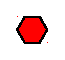
\includegraphics[width=0.5cm]{hexagone2} pour unité d'aire.
 \item Détermine le périmètre de chaque figure colorée, l'unité de longueur sera le côté d'un hexagone.
 \end{enumerate}
 \end{minipage} \hfill%
 \begin{minipage}[c]{0.3\linewidth}
  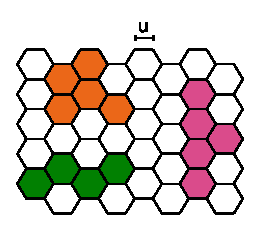
\includegraphics[width=3.7cm]{alveare}
  \end{minipage} \\
\end{partie}

\begin{partie}[Quadrillage triangulaire] \label{PerimAires_act2}
\begin{minipage}[c]{0.5\linewidth}
Mêmes questions que dans la partie \ref{PerimAires_act1}. L'unité d'aire est 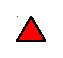
\includegraphics[width=0.45cm]{triangle} et l'unité de longueur le côté d'un triangle.
 \end{minipage} \hfill%
 \begin{minipage}[c]{0.46\linewidth}
  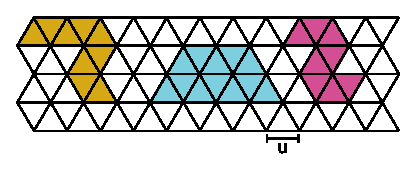
\includegraphics[width=6.2cm]{uniteU}
  \end{minipage} \\
\end{partie}

\begin{partie}
Observe les résultats des questions dans les parties \ref{PerimAires_act1} et \ref{PerimAires_act2} pour répondre aux questions suivantes :
\begin{enumerate}
 \item Les figures ayant la plus grande aire ont‑elles le plus grand périmètre ?
 \item Les figures qui ont le plus petit périmètre ont‑elles la plus petite aire ?
 \end{enumerate}
\end{partie}

\begin{partie}[À toi de jouer]
\begin{enumerate}
 \item Sur du quadrillage, trace plusieurs figures de même aire et compare leurs périmètres ;
 \item Sur du quadrillage, trace plusieurs figures de même périmètre et compare leurs aires.
 \end{enumerate}
\end{partie}

\begin{partie}
\begin{minipage}[c]{0.48\linewidth}
En t'aidant du quadrillage, détermine  approximativement l'aire de la surface délimitée par la ligne orange.
 \end{minipage} \hfill%
 \begin{minipage}[c]{0.48\linewidth}
  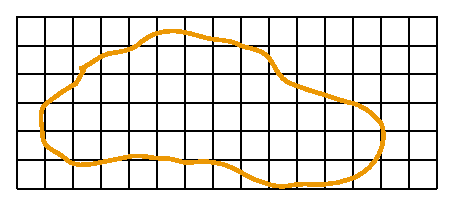
\includegraphics[width=6.8cm]{perimetre_orange}
  \end{minipage} \\
\end{partie}

\end{activite}

%%%%%%%%%%%%%%%%%%%%%%%%%%%%%%%%%%%%%%%%%%%%%%%%%%%%%%%%%%%%%%%%%

\begin{activite}[Unités d'aire]

\begin{center} 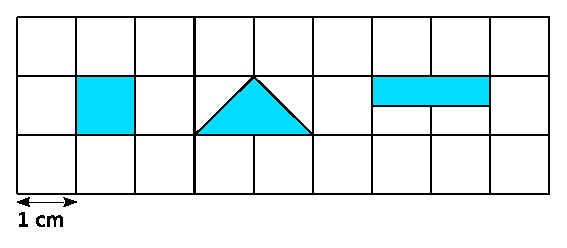
\includegraphics[width=8.5cm]{unites_aire} \end{center}

\begin{partie}
Que peux‑tu dire de l'aire des trois figures bleues ?
\end{partie}

\begin{partie}
L'aire de chacune de ces figures est la même que celle d'un carré de côté 1 cm. On dit que l'aire mesure 1 centimètre carré, on le note 1 cm\up{2}.
\begin{enumerate}
 \item Recopie et complète :
 \begin{center} \textcolor{B2}{Un centimètre carré (cm\up{2}) est la surface occupée par un carré de côté ... .} \end{center}
 \item Définis de la même façon le mètre carré, le décimètre carré, le millimètre carré et le kilomètre carré.
 \end{enumerate}
\end{partie}

\begin{partie}[Ordre de grandeur]
\begin{enumerate}
 \item Quel est l'\textbf{ordre de grandeur} de l'aire d'une page du livre ? Exprime‑la à l'aide de l'unité d'aire la mieux adaptée.
 \item Propose des objets dont l'aire est de l'ordre des unités d'aire les plus usuelles.
 \end{enumerate}
\end{partie}

\begin{partie}[Sur une feuille de papier millimétré]
\begin{enumerate}
 \item Dessine en bleu plusieurs figures dont l'aire est un centimètre carré.
 \item Dessine en rouge un carré d'aire un décimètre carré et en vert un carré d'aire un millimètre carré.
 \item Combien y a‑t‑il de centimètres carrés dans un décimètre carré ?
 \item Combien y a‑t‑il de millimètres carrés dans un centimètre carré ?
 \item Combien y a‑t‑il de millimètres carrés dans un décimètre carré ?
 \end{enumerate}
\end{partie}

\begin{partie}[Aire d'un rectangle]
\begin{minipage}[c]{0.36\linewidth}
\begin{enumerate}
 \item Détermine l'aire du rectangle bleu en centimètres carrés et en millimètres carrés ;
 \item Détermine l'aire du rectangle rouge en millimètres carrés ;
 \item Propose un moyen de déterminer l'aire du rectangle rouge en centimètres carrés.
 \end{enumerate}
 \end{minipage} \hfill%
 \begin{minipage}[c]{0.6\linewidth}
  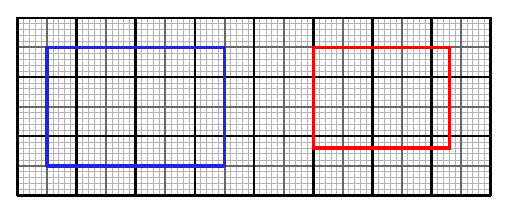
\includegraphics[width=7.6cm]{rectangles}
  \end{minipage} \\
\end{partie}

\begin{partie}
La cour d'un collège est de forme rectangulaire de 75 m sur 35 m :
\begin{enumerate}
 \item Calcule son aire en mètres carrés.
 \item Calcule son aire en décamètres carrés.
 \end{enumerate}
\end{partie}

\begin{partie}
Recherche les dimensions d'un terrain de football, de basket-ball, de tennis et calcule leurs aires respectives en mètres carrés puis en décamètres carrés.
\end{partie}

\end{activite}

%%%%%%%%%%%%%%%%%%%%%%%%%%%%%%%%%%%%%%%%%%%%%%%%%%%%%%%%%%%%%%%%%

\begin{activite}[Du rectangle au parallélogramme]

\begin{enumerate} \label{PerimAires_act3}
\item Construis, sur une feuille, un rectangle de 10 cm de long sur 4 cm de large. Repasse en rouge les longueurs et en vert les largeurs. Calcule l'aire de ce rectangle.


\item Avec un seul coup de ciseaux, découpe le rectangle fait en \ref{PerimAires_act3} puis recolle les morceaux pour obtenir un parallélogramme. Quelle est alors l’aire de ce parallélogramme ?



\item Nadir affirme : « Sur la figure suivante, les quadrilatères $TUCD$, $ABCD$ et $RSCD$ ont la même aire. ». A-t-il raison ? Justifie ta réponse.\\[0.5em]
\begin{center} 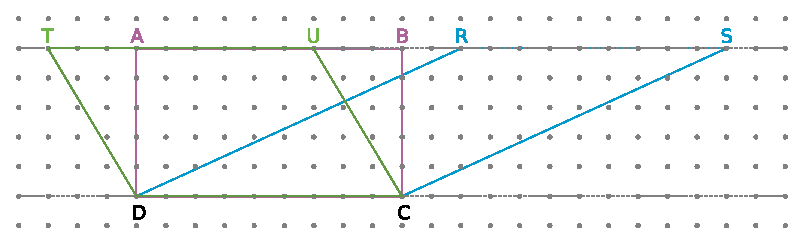
\includegraphics[width=12.4cm]{quadTAUBRS} \end{center}


\item Reproduis sur ton cahier le rectangle $ABCD$ ci-dessus puis prolonge en pointillés les droites $(BC)$ et $(AD)$. Place deux points $E$ et $F$ sur la droite $(AD)$ pour que le parallélogramme $EFBC$ ait la même aire que le rectangle $ABCD$.



\item À l'aide des questions précédentes, propose une ou plusieurs formules qui permettent de calculer l'aire du parallélogramme $EFGH$ ci-dessous.
 
\begin{center}
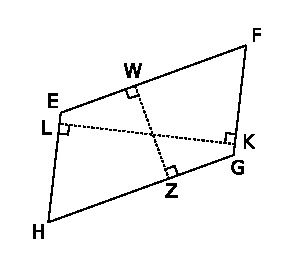
\includegraphics[width=3.6cm]{quadEWF}
\end{center}


\item Rédige une phrase pour expliquer la formule de l'aire d'un parallélogramme.
\end{enumerate}

\end{activite}

%%%%%%%%%%%%%%%%%%%%%%%%%%%%%%%%%%%%%%%%%%%%%%%%%%%%%%%%%%%%%%%%%

\begin{activite}[Perdre sa moitié]

\begin{partie}[Pour un triangle rectangle]
\begin{minipage}[c]{0.56\linewidth}
Le devant du chapeau de Jane est représenté par le croquis ci-contre.

Jeanne veut recouvrir le devant de paillettes pour le carnaval. Sur le tube de paillettes de 5 g, il est écrit qu'il faut 5 g de paillettes pour 20 cm\up{2}. Elle ne sait pas combien de tubes acheter. Elle téléphone à son amie Ipek et lui décrit la forme du chapeau.
 \end{minipage} \hfill%
 \begin{minipage}[c]{0.4\linewidth}
  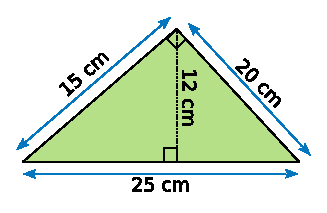
\includegraphics[width=4.8cm]{triangle_vert5}
  \end{minipage} \\
  
Ipek lui répond : « \emph{Pense à un rectangle dont l'aire est le double de ton chapeau.} »

Combien de tubes de paillettes devra acheter Jeanne ?
\end{partie}

\begin{partie}[Pour un triangle quelconque]
\begin{minipage}[c]{0.48\linewidth}
Sur la figure ci-contre, $ABCD$ est un parallélogramme de centre $O$ tel que $AB = 6$ cm et $CH = 2,5$ cm.
\begin{itemize}
 \item Calcule l'aire du parallélogramme $ABCD$.
 \item Que peux-tu observer entre les aires des triangles $ADC$ et $ABC$ ?
 \item Déduis-en l'aire du triangle $ADC$. 
 \end{itemize}
 \end{minipage} \hfill%
 \begin{minipage}[c]{0.48\linewidth}
  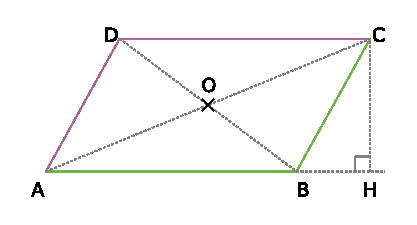
\includegraphics[width=5.5cm]{quad_rosevert}
  \end{minipage} \\[1em]
  Sur la figure ci-dessous, $ABC$ est un triangle tel que $AB = 5$ cm et $CH = 3$ cm. \\[1em]
  \begin{minipage}[c]{0.42\linewidth}
   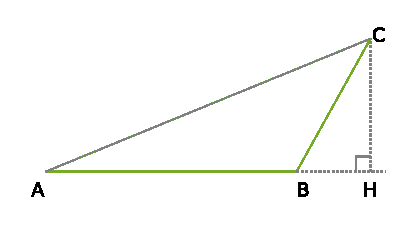
\includegraphics[width=5.4cm]{triangleABCH4} 
   \end{minipage} \hfill%
  \begin{minipage}[c]{0.54\linewidth}
  \begin{itemize}
  \item Dans le triangle $ABC$, que représente la droite $(CH)$ pour le côté $[AB]$ ?
  \item En t’inspirant de la formule de l’aire du parallélogramme, donne une formule permettant de calculer l’aire d’un triangle. 
  \item Combien y a-t-il de façons différentes de calculer l'aire d'un triangle ? Explique ta réponse.
  \end{itemize}
    \end{minipage} \\
\end{partie}

\end{activite}

%%%%%%%%%%%%%%%%%%%%%%%%%%%%%%%%%%%%%%%%%%%%%%%%%%%%%%%%%%%%%%%%%

\newpage

\begin{activite}[En découpant \ldots]

\begin{enumerate}
\item Trace un losange dont les diagonales mesurent $7,5$ cm et $9,6$ cm. Calcule son aire en le découpant de façon à obtenir une figure dont on sait calculer l'aire.

\item Halima a construit un trapèze rectangle de hauteur $4$ cm et dont les deux côtés parallèles mesurent $5$ cm et $8$ cm. Aide-la à calculer l’aire de ce trapèze.

\item Propose une méthode pour calculer l'aire d'un quadrilatère quelconque.
\end{enumerate}

\end{activite}

%%%%%%%%%%%%%%%%%%%%%%%%%%%%%%%%%%%%%%%%%%%%%%%%%%%%%%%%%%%%%%%%%

\begin{activite}[Découpages]

\begin{minipage}[c]{0.76\linewidth}
On considère un carré de côté 6 cm composé de sept polygones particuliers comme l'illustre la figure ci-contre. On sait que le segment rouge mesure $2,2$ cm en vraie grandeur.
 \end{minipage} \hfill%
 \begin{minipage}[c]{0.2\linewidth}
  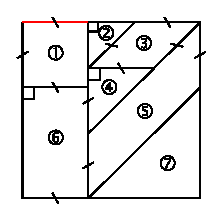
\includegraphics[width=3.1cm]{decoupage1}
  \end{minipage} \\

\begin{enumerate}
\item Précise la nature de chaque polygone puis détermine son aire.

\item Sur une feuille, construis en vraie grandeur le carré et découpe les sept pièces qui le constituent.

\item En assemblant plusieurs de ces pièces, reconstitue chacune des figures suivantes et calcule leur aire :

  \begin{colenumerate}{2}
   \item
   
   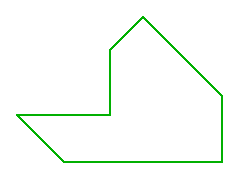
\includegraphics[width=3.3cm]{decoupage2}
   \item
   
   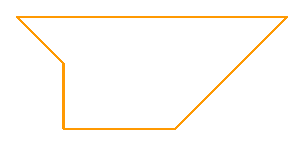
\includegraphics[width=4.4cm]{decoupage3}
   \end{colenumerate}
\end{enumerate}
\end{activite}






\cours
\section{Les 3 dimensions}
\begin{aconnaitre}
Une figure géométrique est représentée en une ou plusieurs dimensions:
\begin{center}
    \begin{tikzpicture} % longueur, surface et volune

%le segment (longueur)
\draw (0,0)--(2,0) node[scale=0.8,midway,above]{longueur} node[scale=0.8,midway,below]{1 dimension};
\draw (0,0)--+(0,0.15)--+(0,-0.15);
\draw (2,0)--+(0,0.15)--+(0,-0.15);

%le carré (surface)
\begin{scope}[xshift=3cm]
\draw[fill=A2] (0,0)--(2,0) node[scale=0.8,midway,below]{2 dimensions} --(2,2) --(0,2) node[scale=0.8,midway,above]{surface} -- cycle;
\end{scope}

%le cube (volume)
\begin{scope}[xshift=8cm]
\def \Width {2};
\def \Height {2};
\def \Depth {2};
\coordinate (O) at (0,0,0);
\coordinate (A) at (0,\Width,0);
\coordinate (B) at (0,\Width,\Height);
\coordinate (C) at (0,0,\Height);
\coordinate (D) at (\Depth,0,0);
\coordinate (E) at (\Depth,\Width,0);
\coordinate (F) at (\Depth,\Width,\Height);
\coordinate (G) at (\Depth,0,\Height);

\draw[blue,fill=blue] (O) -- (C) -- (G) -- (D) -- cycle;% Bottom Face
\draw[blue,fill=A2] (O) -- (A) -- (E) -- (D) -- cycle;% Back Face
\draw[blue,fill=pink] (O) -- (A) -- (B) -- (C) -- cycle;% Left Face
\draw[blue,fill=J1,opacity=0.8] (D) -- (E) -- (F) -- (G) -- cycle;% Right Face
\draw[blue,fill=J2,opacity=0.6] (C) -- (B) -- (F) -- (G) -- cycle;% Front Face
\draw[blue,fill=F,opacity=0.8] (A) -- (B) -- (F) -- (E) -- cycle;% Top Face


\path (C)--(G) node[scale=0.8,midway,below]{3 dimensions};
\path (A)--(E) node[scale=0.8,midway,above]{volume};

%\node at (A) {A};
%\node at (B) {B};
%\node at (C) {C};
%\node at (D) {D};
%\node at (E) {E};
%\node at (F) {F};
%\node at (G) {G};
\end{scope}

\end{tikzpicture}
\end{center}
\end{aconnaitre}


\section{Périmètre d'une figure}
\begin{aconnaitre}[Notion de longueur]
Le mot \MotDefinition{périmètre}{} désigne \textbf{\textcolor{H1}{la longueur}} du contour d'une figure.
\begin{center}
   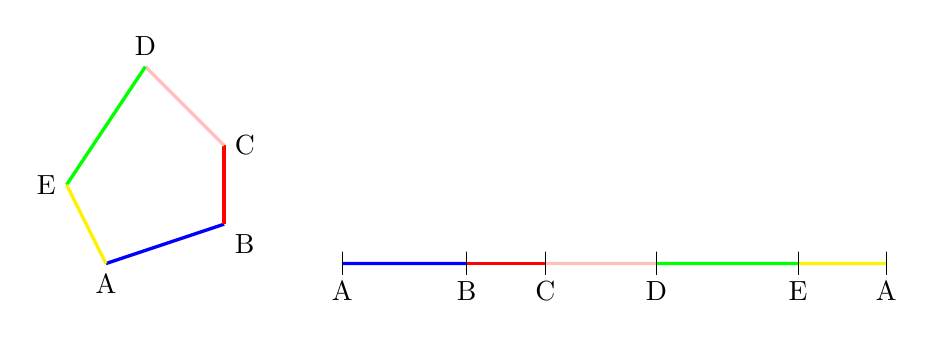
\begin{tikzpicture} % pentagone avec côtés en couleur
\draw [very thick,color=blue] (0,0) node[color=black,below]{A} -- (1.5,0.5) (3,0)--(4.58,0);
\draw [very thick,color=red] (1.5,0.5) node[color=black,below right]{B} -- (1.5,1.5) (4.58,0)--(5.58,0);
\draw [very thick,color=pink] (1.5,1.5) node[color=black,right]{C} -- (0.5,2.5) (5.58,0)--(6.99,0);
\draw [very thick,color=green] (0.5,2.5) node [color=black,above]{D} -- (-0.5,1) (6.99,0)--(8.79,0);
\draw [very thick,color=yellow] (-0.5,1) node[color=black,left]{E} -- (0,0) (8.79,0)--(9.91,0);

\foreach \x / \y in {3/A,4.58/B,5.58/C,6.99/D,8.79/E,9.91/A}
    {\draw (\x,0) node[below=3pt]{\y} --+(0,0.15)--+(0,-0.15);}


\end{tikzpicture} 
\end{center}
Pour exprimer les longueurs, on utilise habituellement pour unité le \textbf{\textcolor{H1}{mètre}} et ses dérivés:
\begin{center}
    \begin{tabular}{|c|c|c|c|c|c|c|}
     \hline   km & hm & dam & m & dm & cm & mm \\ \hline
         & & & & & & \\
    \hline
    \end{tabular}
\end{center}
\end{aconnaitre}

\begin{methode*1}[Transformer des unités de longueurs]

\begin{exemple*1}
Transforme $0,5$ km en m.

Les m (mètres) sont l'unité de mesure.

$1$ km = $\numprint{1000}$ m, donc $0,5$ km $= 0,5 \cdot \numprint{1000}$ m = $500$ m
\end{exemple*1}

\exercice 
Effectue les conversions d'unités de longueur suivantes :
\begin{colenumerate}{3}
 \item $50$ cm en m ;
 \item $100$ mm en m ;
 \item $2,3$ hm en m ;
 \item $0,03$ dm en m ;
 \item $23$ dam en cm ;
 \item $4$ cm en hm.
 \end{colenumerate}
%\correction

\end{methode*1}
%%%%%%%%%%%%%%%%%%%%%%%%%%%%%%%%%%%%%%%%%%%%%%%%%%%%%%%

\section{Aire d'une figure géométrique} 

% remarque : pour qu'un mot se retrouve dans le lexique : \MotDefinition{asymptote horizontale}{} 

\begin{aconnaitre}[Notion de surface]
L' \MotDefinition{aire}{} désigne la valeur de \textbf{\textcolor{H1}{la surface}} occupée par une figure.\\
%le carré
\begin{center}
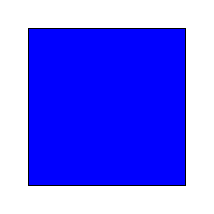
\begin{tikzpicture}
   \begin{scope}[xshift=3cm]
\draw[fill=blue] (0,0)--(2,0) --(2,2) --(0,2) -- cycle;
\end{scope}
\end{tikzpicture}
\end{center}

\prof{
Vous trouverez ici deux lien expliquant le développement du cube et permettant d'expliquer la surface du cube...\\
\href{https://www.geogebra.org/m/arvQstAW}{cube animé}\\
\href{https://www.geogebra.org/m/mZA5qKG9}{patron de cube}
}
Pour exprimer des aires, on utilise habituellement pour unité le \textbf{\textcolor{H1}{mètre carré}} et ses dérivés:
\begin{center}
    \begin{tabular}{|c|c|c|c|c|c|c|c|c|c|c|c|c|c|}
     \hline
     \multicolumn{2}{|c|}{$km^2$} & 
     \multicolumn{2}{c|}{$hm^2$} &
     \multicolumn{2}{c|}{$dam^2$} & 
     \multicolumn{2}{c|}{$m^2$} & 
     \multicolumn{2}{c|}{$dm^2$}  & 
     \multicolumn{2}{c|}{$cm^2$}  & 
     \multicolumn{2}{c|}{$mm^2$}  \\
     \multicolumn{2}{|c|}{} & 
     \multicolumn{2}{c|}{ha} &
     \multicolumn{2}{c|}{a} & 
     \multicolumn{2}{c|}{} & 
     \multicolumn{2}{c|}{}  & 
     \multicolumn{2}{c|}{}  & 
     \multicolumn{2}{c|}{}  \\ \hline
         & & & & & & & & & & & & & \\
    \hline
    \end{tabular}
\end{center}
\end{aconnaitre}

\begin{methode*1}[Pourquoi le tableau des aires comporte des doubles colonnes?]
\begin{exemple*1}\\
Prenons un longueur de 1$cm$.
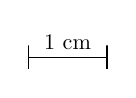
\begin{tikzpicture} %segment de 1cm
\draw (0,0)--(1,0) node[scale=0.8,midway,above]{1 cm};
\draw (0,0)--+(0,0.15)--+(0,-0.15);
\draw (1,0)--+(0,0.15)--+(0,-0.15);
\end{tikzpicture}

Formons une surface basée sur sur cette longueur:
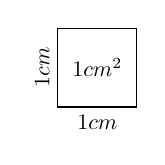
\begin{tikzpicture}%carré de 1cm^2
\draw (0,0)--(1,0) node[scale=0.8,midway,below]{$1 \text{cm}$} --(1,1) --(0,1) -- cycle;
\node[scale=0.8,rotate=90] at(-0.2,0.5) {$1 \text{cm}$};
\node[scale=0.8] at (0.5,0.5) {$1 \text{cm}^2$};
\end{tikzpicture}

L'aire de cette figure est de 1$cm^2$. \\

Maintenant, prenons une longueur dix fois plus grande c'est à dire 10$cm$ soit 1$dm$.\\
\begin{tikzpicture} %segment de 10cm
\draw (0,0)--(10,0) node[scale=0.8,midway,above]{10 cm} node[scale=0.8,midway,below]{1 dm};
\draw (0,0)--+(0,0.15)--+(0,-0.15);
\draw (10,0)--+(0,0.15)--+(0,-0.15);
\end{tikzpicture}

Formons une surface basée sur cette longueur:\\
\begin{tikzpicture}%carré de 100cm^2
\draw (0,0)--(10,0) node[scale=0.8,midway,below]{$10 \text{cm}$} --(10,10) --(0,10) -- cycle;
\node[scale=0.8,rotate=90] at(-0.2,5) {$10 \text{cm}$};
\node[scale=0.8] at (5,5) {$100 \text{cm}^2=1\text{dm}^2$};
\end{tikzpicture}

L'aire est alors de 100$cm^2$.\\
Que remarque-t-on?\\
Lorsqu'une longueur est multipliée par 10, l'aire qui lui est relative est multipliée par 100.\\
La double colonne dans le tableau des aires permet de retranscrire ce phénomène.
\end{exemple*1}
\exercice
Effectue les conversions d'unités d'aire suivantes:
\begin{colenumerate}{3}
 \item $7$ dm\up{2} en m\up{2} ;
 \item $200$ cm\up{2} en m\up{2} ;
 \item $3,2$ ha en m\up{2} ;
 \item $0,8$ dm\up{2} en m\up{2} ;
 \item $45$ hm\up{2} en dm\up{2} ;
 \item $400$ cm\up{2} en a.
 \end{colenumerate}
\end{methode*1}



\begin{methode*1}[Évaluer une aire]
\begin{exemple*1}
\begin{minipage}[c]{0.55\textwidth}
 À l'aide du quadrillage, détermine un encadrement de l'aire de la surface jaune, en prenant pour unité un carreau bleu.
 \end{minipage} \hfill%
 \begin{minipage}[c]{0.2\textwidth}
 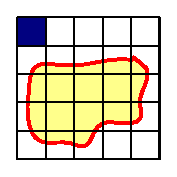
\includegraphics[width=2.3cm]{aire1}
 \end{minipage} \\
 
 \begin{minipage}[c]{0.1\textwidth}
  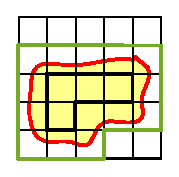
\includegraphics[width=2.3cm]{aire2}
 \end{minipage} \hfill%
 \begin{minipage}[c]{0.7\textwidth}
La surface délimitée en \textbf{\textcolor{H1}{vert}} a une aire plus grande que celle délimitée par la courbe rouge. On compte le nombre de carreaux. Son aire est 18 carreaux.
 \end{minipage} \\[1em]
La surface délimitée en \textbf{noir} a une aire plus petite que celle délimitée par la courbe rouge. On compte le nombre de carreaux. Son aire est quatre carreaux.

Donc l'aire de la figure jaune est comprise entre 4 et 18 carreaux.

\end{exemple*1}

\exercice 
\begin{minipage}[c]{0.50\textwidth}
 Détermine l'aire, en nombre de carrés, des deux figures ci-contre.
 \end{minipage} \hfill%
 \begin{minipage}[c]{0.16\textwidth}
 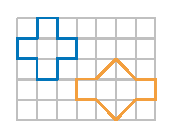
\includegraphics[width=2.2cm]{aire3}
 \end{minipage} \\
%\correction
 
\end{methode*1}

%%%%%%%%%%%%%%%%%%%%%%%%%%%%%%%%%%%%%%%%%%%%%%%%%%%%%%%

\prof{
\begin{activite}[Problème à Dudu: peindre le cabanon]
\begin{partie}[objectif]
A ce stade, les élèves ne connaissent pas encore les formules de calcul d'aire. Le but est de leur faire découvrir par nécessité. Pour ce faire, ils peuvent avoir accès à différentes ressources bien que tout soit dans le livre.
\end{partie}
\begin{partie}[Mise en place]
Mettre les élèves par groupe de 4 environ.
\end{partie}

\begin{partie}[Consigne]
"on va regarder une vidéo. Tout est indiqué dans le film. Vous allez travailler ensemble pour essayer de répondre à la question qui va vous être posée". Chaque groupe devra rendre son travail qui explique clairement sa démarche sur une feuille A3 (et éventuellement la présenter à la classe!).\\
\end{partie}

\begin{partie}[La vidéo]
Voici le lien qui mène vers la vidéo:
\href{https://www.youtube.com/watch?v=ALUiqD4blG8}{Peindre le cabanon}.
On peut diffuser la vidéo à plusieurs reprises si nécessaire mais il est important que les élèves finissent par prendre des notes.
\end{partie}

\begin{partie}[Déroulement]
Après avoir regardé la vidéo 2 ou 3 fois, les élèves se mettent au travail.\\
Très vite, ils vont avoir besoin de formules qu'ils ne connaissent pas nécessairement. On peut alors les orienter vers les pages du livre correspondantes ou imaginer un prolongement à l'activité avec une tablette ou des ressources mises à disposition dans la classe.\\

Quand les élèves ont terminé, on peut imaginer une rapide présentation de leur travail à la classe. On peut afficher les travaux ou les noter...\\

Voici le genre de travail attendu....:
\begin{center}
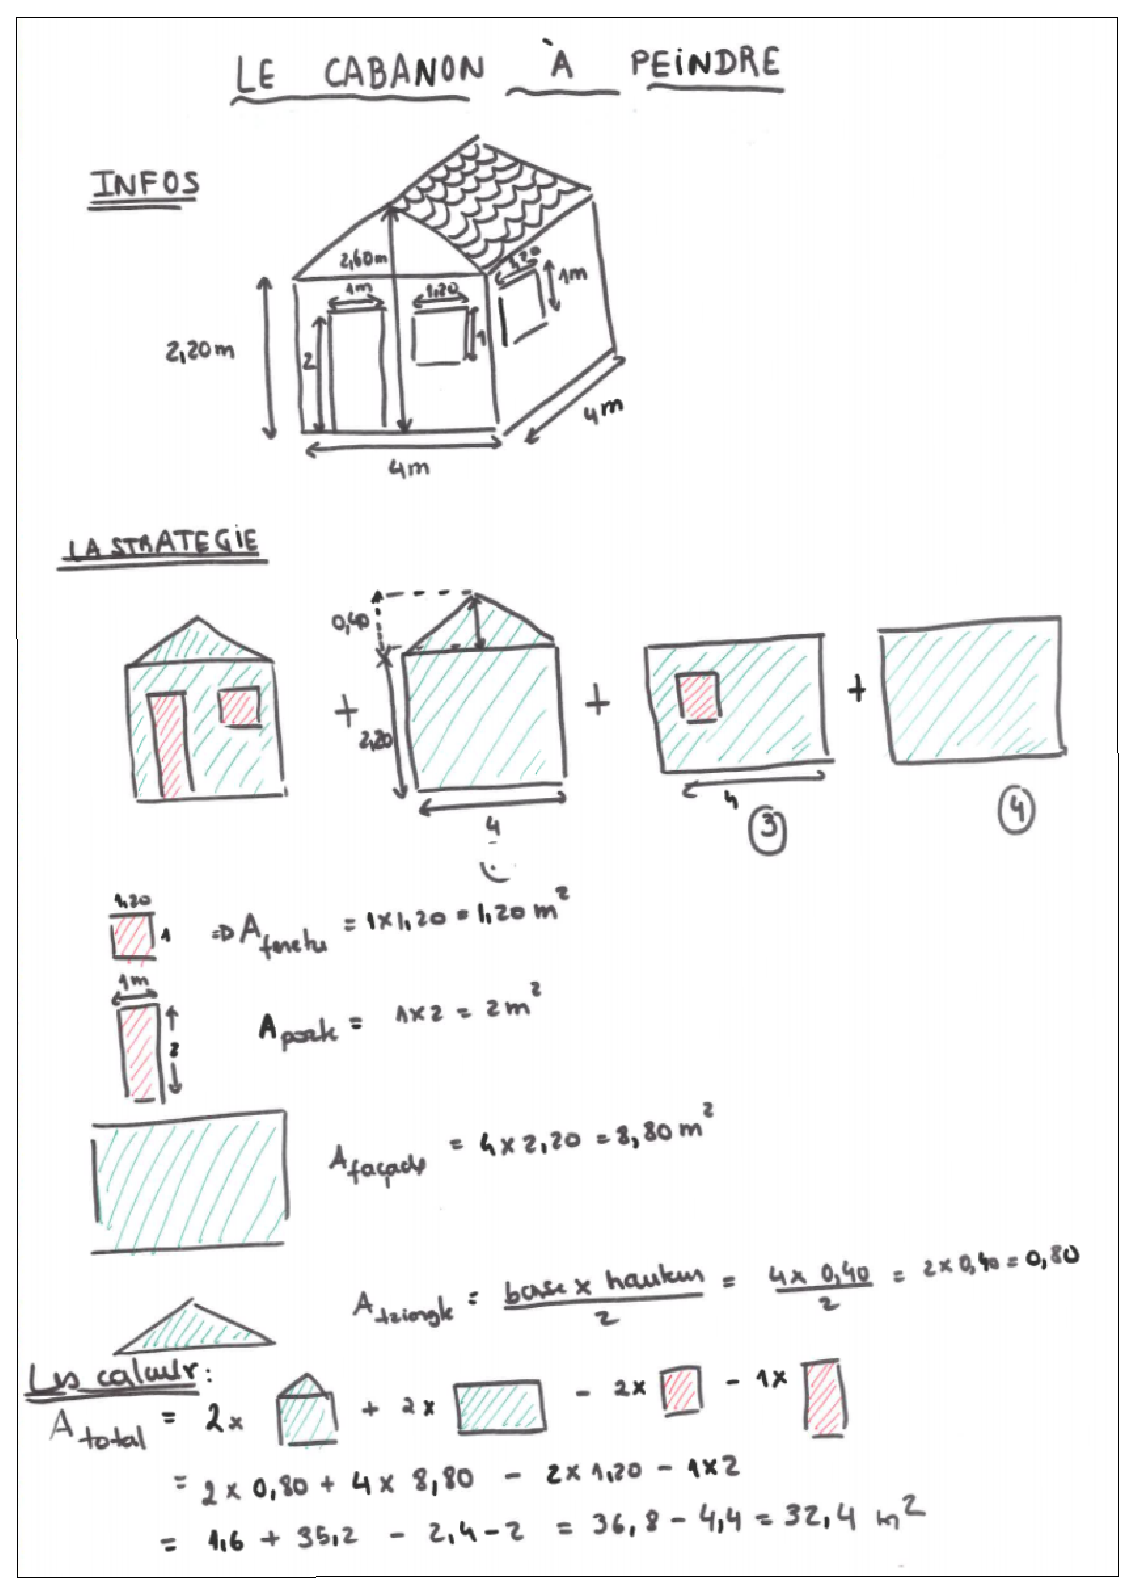
\includegraphics[width=14cm]{PerimetresAires/figures/cabanon.eps} 
\end{center}

\end{partie}
\end{activite}
}

%%%%%%%%%%%%%%%%%%%%%%%%%%%%%%%%%%%%%%%%%%%%%%%%%%%%%%%

\section{Volume d'un solide}

\begin{aconnaitre}[Notion de volume]
Le mot \MotDefinition{volume}{} désigne l'espace contenu dans une figure en 3 dimensions.\\
Pour exprimer des volumes, on utilise habituellement pour unité le \textbf{\textcolor{H1}{mètre cube}} et ses dérivés:
\begin{center}
    \begin{tabular}{|c|c|c|c|c|c|c|c|c|c|c|c|c|c|c|c|c|c|c|c|c|}
     \hline
     \multicolumn{3}{|c|}{$km^3$} & 
     \multicolumn{3}{c|}{$hm^3$} &
     \multicolumn{3}{c|}{$dam^3$} & 
     \multicolumn{3}{c|}{$m^3$} & 
     \multicolumn{3}{c|}{$dm^3$}  & 
     \multicolumn{3}{c|}{$cm^3$}  & 
     \multicolumn{3}{c|}{$mm^3$}  \\    \hline
         & & & & & & & & & & & & & & & & & & & & \\
    \hline
    \end{tabular}
\end{center}
\end{aconnaitre}

\begin{methode*1}[Pourquoi le tableau des volumes comporte des triples colonnes?]
\begin{exemple*1}\\
On a vu précédemment que lorsque la longueur d'un carré est multipliée par 10, son aire est multipliée par 100.\\
Il en va de même avec les volumes. Lorsque la longueur d'un cube est multipliée par 10, le volume se trouve multiplié par 1000. C'est pour retranscrire ce phénomène que le tableau des volumes comporte des triples colonnes.
\end{exemple*1}
\exercice
Effectue les conversions d'unités de volume suivantes:
\begin{colenumerate}{3}
 \item $7,61$ km\up{3} en hm\up{3} ;
 \item $5,15$ m\up{3} en cm\up{3} ;
 \item $8,12$ cm\up{3}  en dm\up{3} ;
 \item $12,1$ m\up{3} en hm\up{3} ;
 \item $85,3$ hm\up{3} en dam\up{3} ;
 \item $48,7$ dam\up{3} en m\up{3}.
 \end{colenumerate}
\end{methode*1}


%%%%%%%%%%%%%%%%%%%%%%%%%%%%%%%%%%%%%%%%%%%%%%%%%%%%%%%%%%%%%%%%%
\begin{center}
    \textsc{\textbf{POUR RÉSUMER...}}\\
    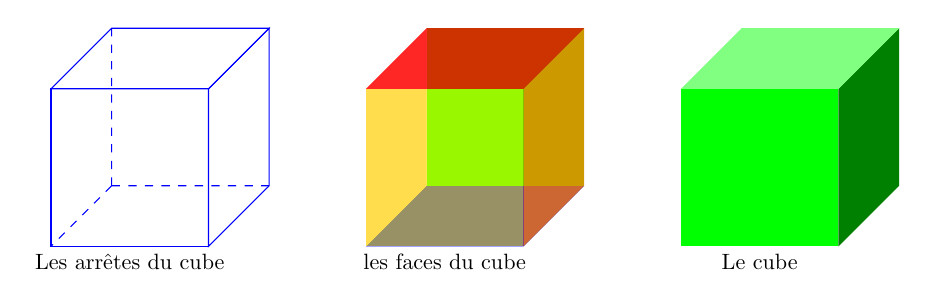
\begin{tikzpicture} 
\def \Width {2};
\def \Height {2};
\def \Depth {2};

%les arrêtes du cube
\begin{scope}
\def \translate {0};
\coordinate (O) at (0+\translate,0,0);
\coordinate (A) at (0+\translate,\Width,0);
\coordinate (B) at (0+\translate,\Width,\Height);
\coordinate (C) at (0+\translate,0,\Height);
\coordinate (D) at (\Depth+\translate,0,0);
\coordinate (E) at (\Depth+\translate,\Width,0);
\coordinate (F) at (\Depth+\translate,\Width,\Height);
\coordinate (G) at (\Depth+\translate,0,\Height);

\draw[dashed, blue] (O) -- (A) (O) -- (C) (O) -- (D);% arrêtes cachées
\draw[blue] (D) -- (E) -- (F) -- (G) -- cycle;% Right Face
\draw[blue] (C) -- (B) -- (F) -- (G) -- cycle;% Front Face
\draw[blue] (A) -- (B) -- (F) -- (E) -- cycle;% Top Face

\path (C)--(G) node[scale=0.8,midway,below]{Les arrêtes du cube};

%\node at (A) {A};
%\node at (B) {B};
%\node at (C) {C};
%\node at (D) {D};
%\node at (E) {E};
%\node at (F) {F};
%\node at (G) {G};
\end{scope}

%les faces du cubes
\begin{scope}
\def \translate {4};

\coordinate (O) at (0+\translate,0,0);
\coordinate (A) at (0+\translate,\Width,0);
\coordinate (B) at (0+\translate,\Width,\Height);
\coordinate (C) at (0+\translate,0,\Height);
\coordinate (D) at (\Depth+\translate,0,0);
\coordinate (E) at (\Depth+\translate,\Width,0);
\coordinate (F) at (\Depth+\translate,\Width,\Height);
\coordinate (G) at (\Depth+\translate,0,\Height);

\fill[blue] (O) -- (C) -- (G) -- (D) -- cycle;% Bottom Face
\fill[green] (O) -- (A) -- (E) -- (D) -- cycle;% Back Face
\fill[pink] (O) -- (A) -- (B) -- (C) -- cycle;% Left Face
\fill[orange,opacity=0.8] (D) -- (E) -- (F) -- (G) -- cycle;% Right Face
\fill[yellow,opacity=0.6] (C) -- (B) -- (F) -- (G) -- cycle;% Front Face
\fill[red,opacity=0.8] (A) -- (B) -- (F) -- (E) -- cycle;% Top Face


\path (C)--(G) node[scale=0.8,midway,below]{les faces du cube};
%\path (A)--(E) node[scale=0.8,midway,above]{solide (ou volume?)};

%\node at (A) {A};
%\node at (B) {B};
%\node at (C) {C};
%\node at (D) {D};
%\node at (E) {E};
%\node at (F) {F};
%\node at (G) {G};
\end{scope}

%le cube
\begin{scope}
\def \translate {8};

\coordinate (O) at (0+\translate,0,0);
\coordinate (A) at (0+\translate,\Width,0);
\coordinate (B) at (0+\translate,\Width,\Height);
\coordinate (C) at (0+\translate,0,\Height);
\coordinate (D) at (\Depth+\translate,0,0);
\coordinate (E) at (\Depth+\translate,\Width,0);
\coordinate (F) at (\Depth+\translate,\Width,\Height);
\coordinate (G) at (\Depth+\translate,0,\Height);

%\draw (O) -- (C) -- (G) -- (D) -- cycle;% Bottom Face
%\draw (O) -- (A) -- (E) -- (D) -- cycle;% Back Face
%\draw (O) -- (A) -- (B) -- (C) -- cycle;% Left Face
\fill[green!50!black] (D) -- (E) -- (F) -- (G) -- cycle;% Right Face
\fill[green] (C) -- (B) -- (F) -- (G) -- cycle;% Front Face
\fill[green!50!white] (A) -- (B) -- (F) -- (E) -- cycle;% Top Face


\path (C)--(G) node[scale=0.8,midway,below]{Le cube};
%\path (A)--(E) node[scale=0.8,midway,above]{solide (ou volume?)};

%\node at (A) {A};
%\node at (B) {B};
%\node at (C) {C};
%\node at (D) {D};
%\node at (E) {E};
%\node at (F) {F};
%\node at (G) {G};
\end{scope}


\end{tikzpicture}

\end{center}

%%%%%%%%%%%%%%%%%%%%%%%%%%%%%%%%%%%%%%%%%%%%%%%%%%%%%%%%%%%%%%%%%

\newpage

\vspace{2em}
\section{Calculer des aires à l'aide d'une formule}

\begin{aconnaitre}[aire du rectangle et du triangle rectangle]
\begin{tabularx}{\linewidth}{|c|X|X|}
 \cline{2-3}
\multicolumn{1}{c|}{} & \begin{center} \textbf{\textcolor{H1}{Rectangle}} 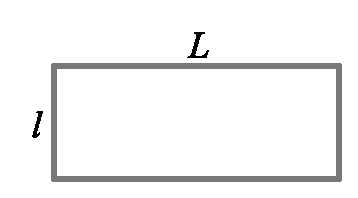
\includegraphics[width=2.5cm]{rectangleLI} \end{center} & \begin{center} \textbf{\textcolor{H1}{Triangle rectangle}} 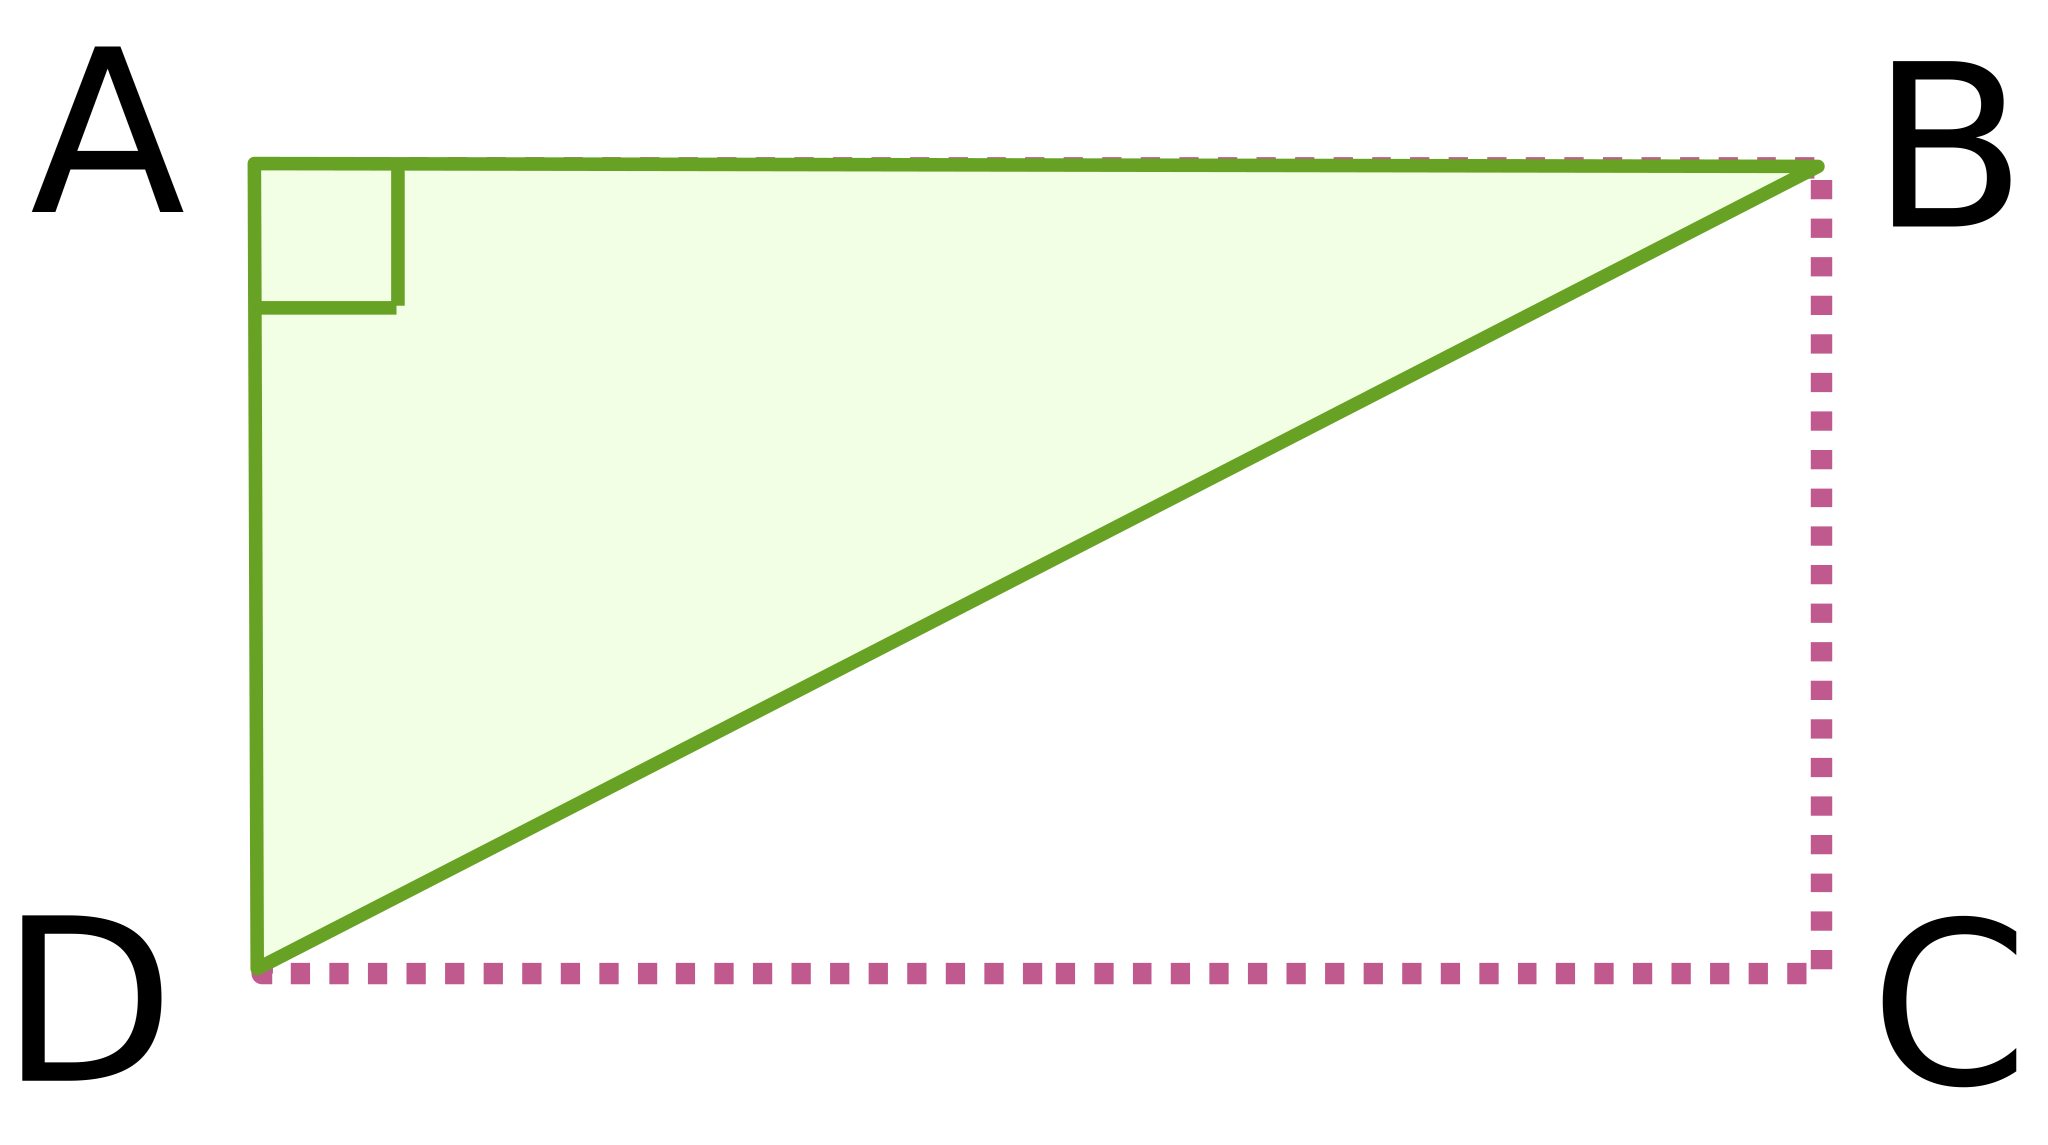
\includegraphics[width=2.7cm]{rectangleABCD4} \end{center} \\ \hline
Formule & L'aire du rectangle peut se calculer avec cette formule : {\large \textbf{$\mathcal{A} = L \cdot \ell$}} & L'aire de $ABD$ est égale à la moitié de l'aire de $ABCD$ : {\large \textbf{$\mathcal{A} = \dfrac{AB \cdot AD}{2}$}} \phantom{retourligne} \\\hline
 \end{tabularx} \\[1em]
Les longueurs doivent être exprimées dans la même unité.
\end{aconnaitre}
\begin{methode*1}
\begin{exemple*1}
Calcule l'aire de la figure $ABCDE$ ci‑dessous (L'unité de longueur est le centimètre) :
\begin{center}  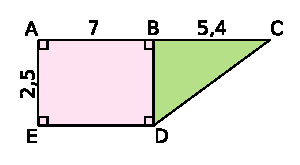
\includegraphics[width=4.3cm]{aire4} \end{center}

 \begin{itemize}
  \item La figure est composée du rectangle $ABDE$ et du triangle rectangle $BCD$. Son aire est donc égale à la somme de l'aire de $ABDE$ et de l'aire de $BCD$ ;
  \item $\mathcal{A}_{ABDE} = AB \cdot AE = 7$ cm $\cdot$ $2,5$ cm = $17,5$ cm\up{2} ; \\[0.2em]
  \item $\mathcal{A}_{BCD} = \dfrac{BC \cdot BD}{2} = \dfrac{5,4 \text{ cm} \cdot 2,5 \text{ cm}}{2} = \dfrac{13,5 \text{ cm}\up{2}}{2} = 6,75 $ cm\up{2} ;\\[0.2em]
  \item $\mathcal{A}_{ABCDE} = 17,5$ cm\up{2} $+ 6,75$ cm\up{2} = $24,25$ cm\up{2}.
  \item L'aire de la figure $ABCDE$ est donc égale à $24,25$ cm\up{2}.
  \end{itemize}
\end{exemple*1}

\exercice 
Détermine l'aire d'un carré de côté 6 cm. 
%\correction

\exercice 
Détermine l'aire d'un rectangle de longueur 3 cm et de largeur 22 mm en donnant le résultat en cm\up{2}.
%\correction
     
\exercice 
$SON$ est un triangle rectangle en $S$, tel que 

$SO = 8,04$ dm et $SN = 0,93$ m. Détermine son aire en donnant le résultat en m\up{2}.
%\correction
 
\end{methode*1}
%%%%%%%%%%%%%%%%%%%%%%%%%%%%%%%%%%%%%%%%%%%%%%%%%%%%%%%%
\newpage

\vspace{2em}

\begin{aconnaitre}[Aire d'un triangle]
Pour calculer l’aire d’un triangle, on multiplie la \textbf{\textcolor{H1}{longueur d'un côté}} par la \textbf{\textcolor{C2}{hauteur}} relative à ce côté puis on divise le résultat par 2 :

\begin{tabularx}{\textwidth}{XX}
{\large $\mathcal{A} = \dfrac{b \cdot h}{2}$} & 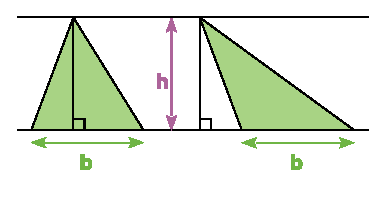
\includegraphics[width=5cm]{longueur_hauteur} \\
 \end{tabularx} \\
 \end{aconnaitre}

\vspace{4em}

\begin{methode*1}[Calculer l’aire d’un triangle]


 
\begin{exemple*1}
Calcule l’aire du triangle suivant :
\begin{minipage}[c]{0.68\textwidth}
\begin{itemize}
 \item On mesure la longueur d'un côté ;
 \item On mesure la hauteur relative à ce côté ;
 \item On multiplie la longueur du côté repéré par la hauteur relative à ce côté puis on divise le résultat par 2 : \\[0.3em]
$\mathcal{A} = \dfrac{10 \cdot 3}{2} = \dfrac{30}{2} = 15$. \\[0.3em]
L'aire du triangle vaut 15 cm\up{2}.
 \end{itemize}
 \end{minipage} \hfill%
 \begin{minipage}[c]{0.2\textwidth}
 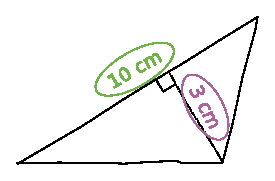
\includegraphics[width=3.5cm]{triangle_croquisZ}
 \end{minipage} \\
\end{exemple*1}


\exercice 
Calcule l’aire des triangles suivants :
\begin{colenumerate}{2}
 \item
 
 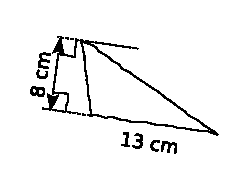
\includegraphics[width=3.1cm]{triangle_croquisY}
 \item
 
 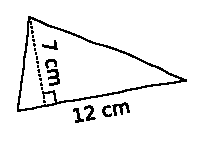
\includegraphics[width=2.8cm]{triangle_croquisW}
 \end{colenumerate}
%\correction

\end{methode*1}
%%%%%%%%%%%%%%%%%%%%%%%%%%%%%%%%%%%%%%%%%%%%%%%%%%%%%%%%
\newpage

\vspace{2em}

\begin{aconnaitre}[Aire d'un parallélogramme]
Pour calculer l’\MotDefinition{aire d’un parallélogramme}{}, on multiplie la \textbf{\textcolor{H1}{longueur d'un côté}} par la \textbf{\textcolor{C2}{hauteur}} relative à ce côté :

\vspace{1em}

\begin{tabularx}{\textwidth}{XX}
{\large $\mathcal{A} = b \cdot h$} & 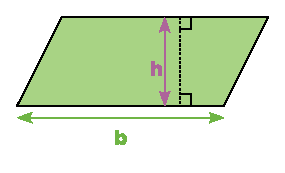
\includegraphics[width=4cm]{parallelogrammehb} \\
 \end{tabularx} \\

\end{aconnaitre}


\vspace{4em}

\begin{methode*1}[Calculer l’aire d’un parallélogramme]


\begin{exemple*1}
Détermine l’\textbf{aire} du parallélogramme suivant :
\begin{minipage}[c]{0.65\textwidth}
\begin{itemize}
 \item On mesure la \textbf{\textcolor{H1}{longueur}} d'un côté ;
 \item On mesure la \textbf{\textcolor{C2}{hauteur}} relative à ce côté ;
 \item On multiplie la longueur du côté repéré par la hauteur relative à ce côté : $\mathcal{A} = 12 \cdot 5 = 60$ ;
 \item L'aire du parallélogramme vaut 60 cm\up{2}.
 \end{itemize}
 \end{minipage} \hfill%
 \begin{minipage}[c]{0.26\textwidth}
 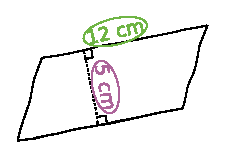
\includegraphics[width=3cm]{parallelog_croquis}
 \end{minipage} \\
\end{exemple*1}

\exercice 
Détermine l’aire des parallélogrammes $MNOP$ et $ABCD$ ci-dessous :
\begin{colenumerate}{2}
 \item 
 
 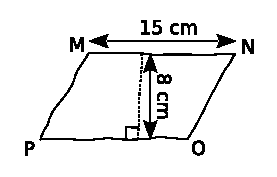
\includegraphics[width=3.7cm]{parallelogMNPO}
 \item 
 
 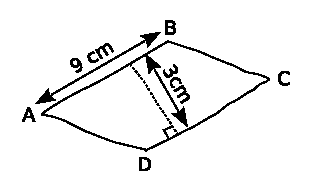
\includegraphics[width=4.4cm]{parallelogABCD}
 \end{colenumerate}
%\correction

\end{methode*1}
%%%%%%%%%%%%%%%%%%%%%%%%%%%%%%%%%%%%%%%%%%%%%%%%%%%%%%%%



\newpage

\vspace{2em}

\begin{aconnaitre}[Aire d'un losange]
Pour calculer l’aire d’un losange, on effectue le produit des \textbf{\textcolor{H1}{longueurs des diagonales}} puis on divise le résultat par 2 : 

\begin{tabularx}{\textwidth}{XX}
{\large $\mathcal{A} = \dfrac{d \cdot D}{2}$} & 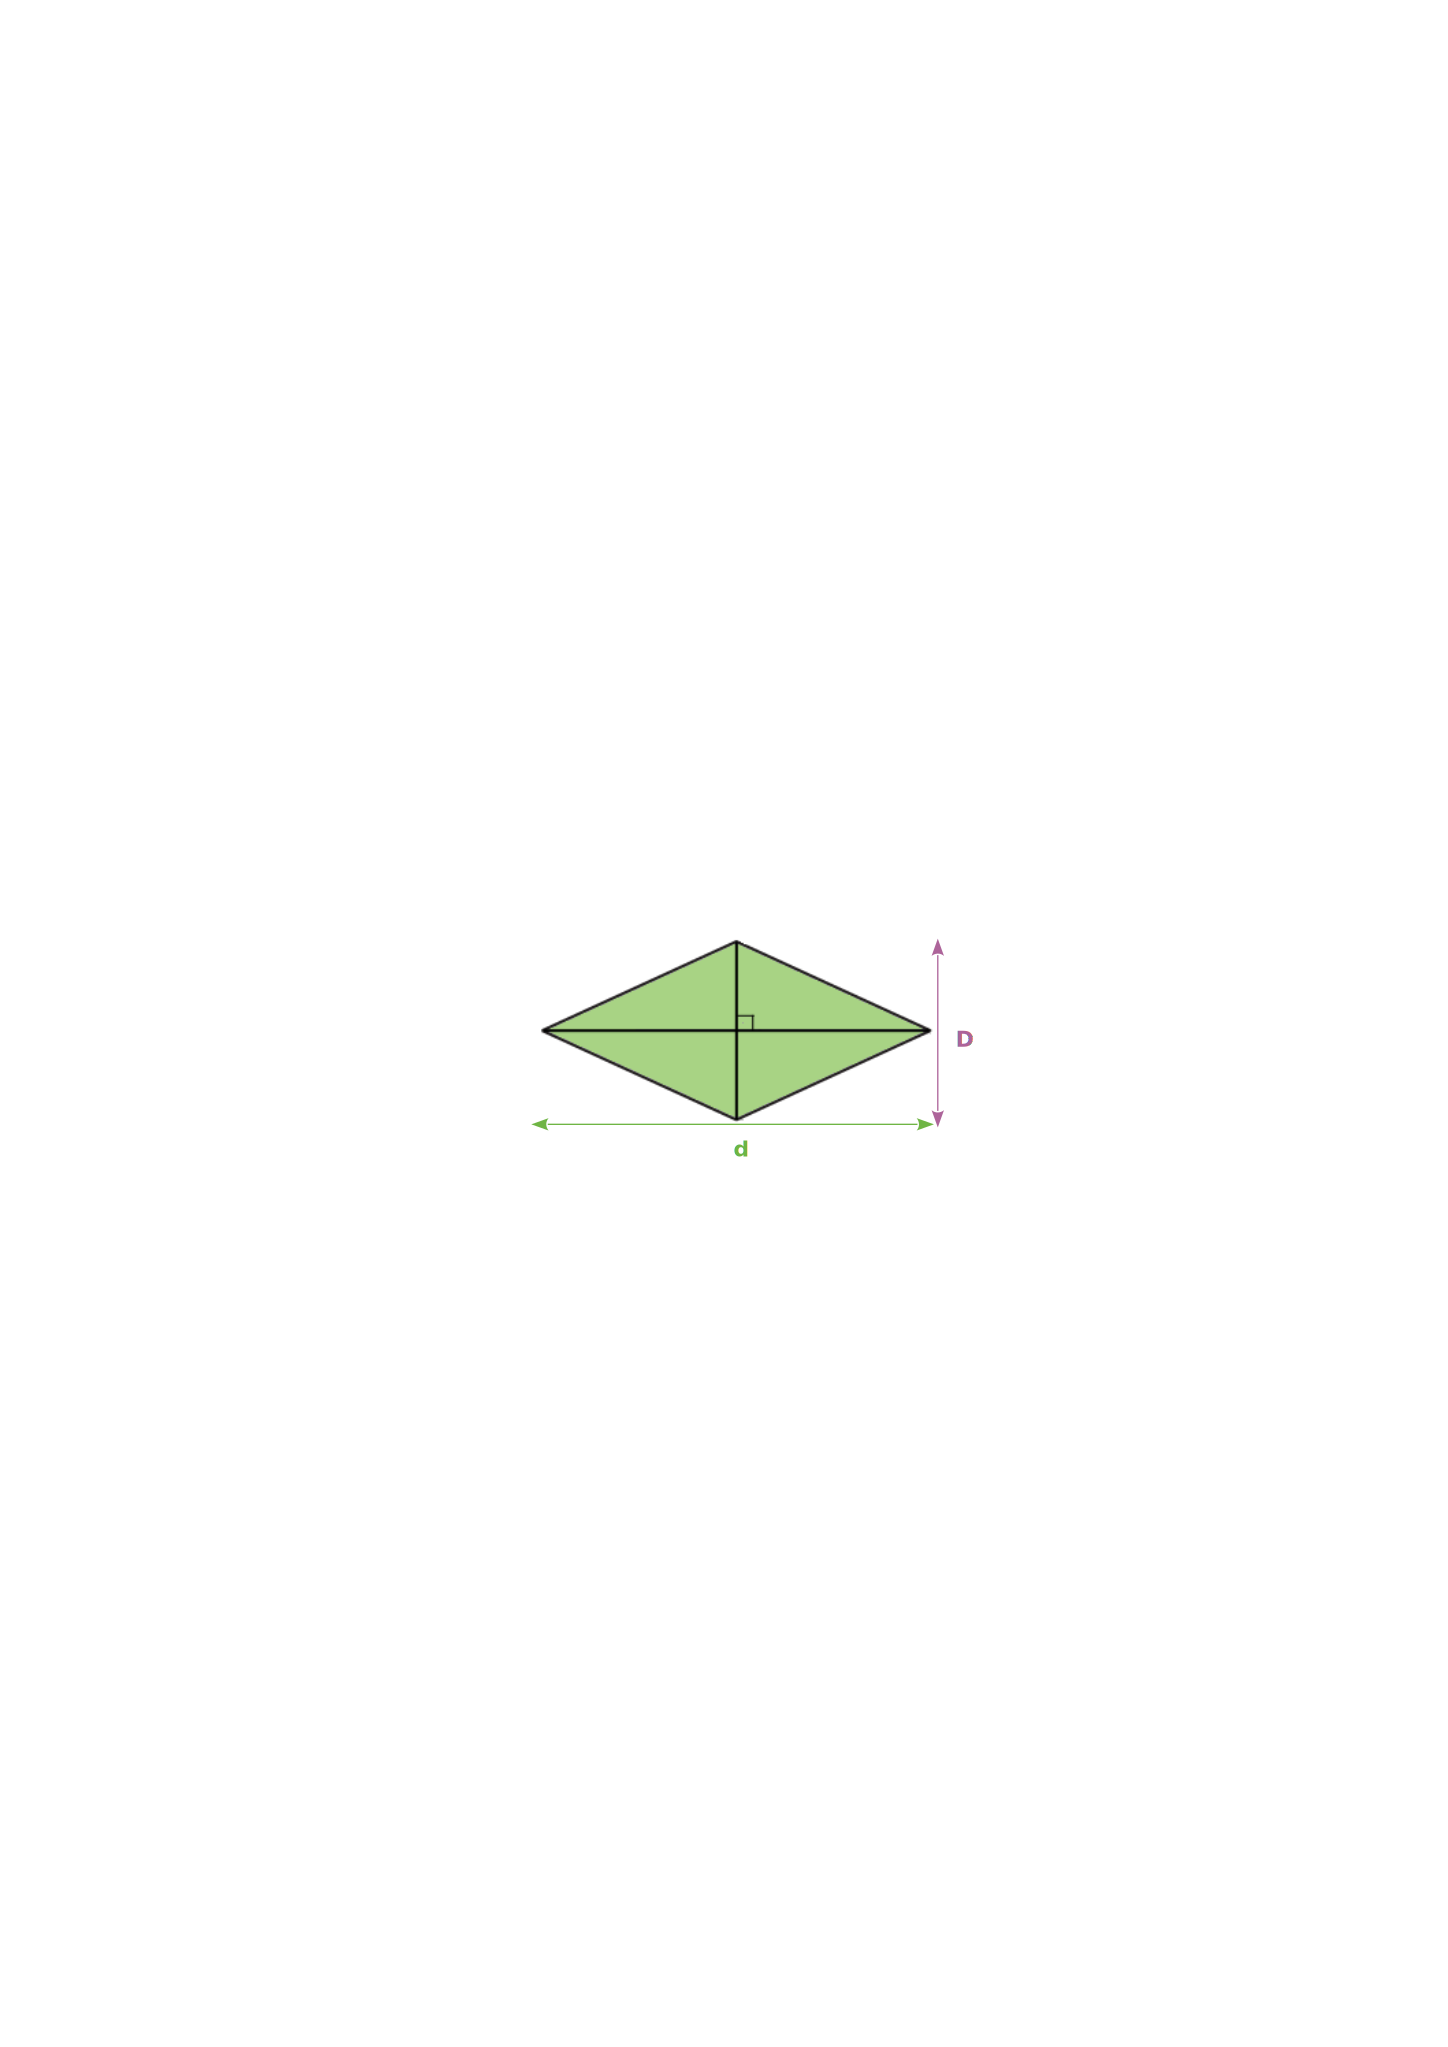
\includegraphics[width=5cm]{losangeDd} \\
 \end{tabularx} \\
 \end{aconnaitre}

\vspace{4em}

\begin{methode*1}[Calculer l’aire d’un losange]


 
 \begin{exemple*1}
Calcule l’aire du losange suivant :
\begin{minipage}[c]{0.68\textwidth}
\begin{itemize}
 \item On repère la longueur des diagonales.
 \item On calcule le produit des longueurs des diagonales puis on divise le résultat par 2 : \\[0.3em]
$\mathcal{A} = \dfrac{10 \cdot 5}{2} = \dfrac{50}{2} = 25$ \\[0.3em]
L'aire du losange vaut 25 cm\up{2}.
 \end{itemize}
 \end{minipage} \hfill%
 \begin{minipage}[c]{0.2\textwidth}
 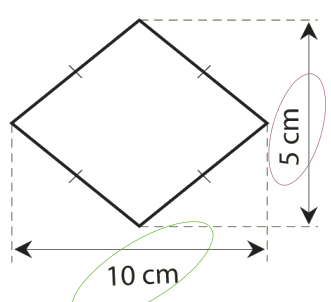
\includegraphics[width=2.9cm]{losange26}
 \end{minipage} \\
\end{exemple*1}

 
 \exercice
Calcule l’aire des losanges suivants :
\begin{colenumerate}{2}
 \item
 
 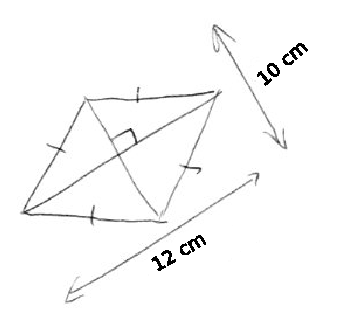
\includegraphics[width=5cm]{losange12_10}
 \item
 
 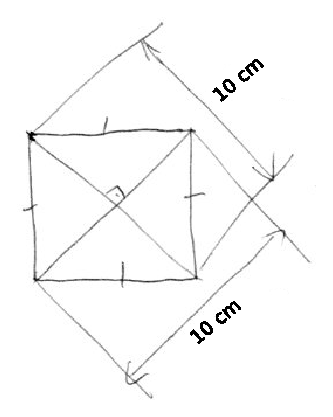
\includegraphics[width=4cm]{losange10_10}
 \end{colenumerate}
%\correction

\end{methode*1}



\exercicesbase
\begin{colonne*exercice}

\serie{Conversions}

\begin{exercice}
Convertis les longueurs :
\begin{enumerate}
 \item $5$ mm = \ldots \ldots \ldots m ;
 \item $2,8$ hm = \ldots \ldots \ldots km ;
 \item $3$ dam = \ldots \ldots \ldots m ;
 \item $3,8$ dm = \ldots \ldots \ldots cm.
 \end{enumerate}
\end{exercice}


\begin{exercice}
Convertis dans l’unité demandée :
\begin{itemize}
 \item $\numprint{4405}$ m = \dotfill dam ;
 \item $0,007$ dam = \dotfill mm ;
 \item $45,3$ hm = \dotfill m ;
 \item $\numprint{12352}$ cm = \dotfill m ;
 \item $0,542$ km = \dotfill dm ;
 \item $7,03$ hm = \dotfill cm ;
 \item $\numprint{17005}$ cm = \dotfill km ;
 \item $123,5$ m = \dotfill km ;
 \item $0,045$ dam = \dotfill hm ;
 \item $\numprint{10000}$ mm =	\dotfill dam ;
 \item $6$ km $+ 12$ dam $+ 9$ m = \dotfill hm.
 \end{itemize}
\end{exercice}


\begin{exercice}
Pour aller au collège, Caroline fait d'abord 1,4 km avec son vélo qu'elle laisse chez sa grand‑mère. Puis elle parcourt les 150 m restant à pied. Quelle distance totale parcourt‑elle ?
\end{exercice}


\begin{exercice}
Recopie et complète :
\begin{enumerate}
 \item $4$ dam\up{2} = \ldots \ldots \ldots m\up{2} ;
 \item $15$ hm\up{2} = \ldots \ldots \ldots m\up{2} ;
 \item $5,1$ cm\up{2} = \ldots \ldots \ldots mm\up{2} ;
 \item $\numprint{1350}$ mm\up{2} = \ldots \ldots \ldots cm\up{2} ;
 \item $5,2$ km\up{2} = \ldots \ldots \ldots m\up{2} ;
 \item $0,7$ m\up{2} = \ldots \ldots \ldots dam\up{2} ;
 \item $320$ a = \ldots \ldots \ldots m\up{2} ;
 \item $2,5$ ha = \ldots \ldots \ldots m\up{2} ;
 \item $\numprint{15300}$ mm\up{2} = \ldots\ldots cm\up{2} =  \ldots\ldots dm\up{2} = \ldots\ldots m\up{2}.
 \end{enumerate}
\end{exercice}


\begin{exercice}
Convertis les aires suivantes en m\up{2} :
\begin{colenumerate}{3}
 \item $2$ km\up{2} ;
 \item $\numprint{37000}$ dm\up{2} ;
 \item $\numprint{45300}$ mm\up{2} ;
 \item $153,7$ dam\up{2} ;
 \item $28,9$ cm\up{2} ;
 \item $3,008$ hm\up{2} ;
 \item $52$ a ;
 \item $0,05$ ha ;
 \item $200$ ha.
 \end{colenumerate}
\end{exercice}


\begin{exercice}
Convertis les aires suivantes en cm\up{2} :
\begin{colenumerate}{3}
 \item $15$ mm\up{2} ;
 \item $28$ dm\up{2} ;
 \item $\numprint{17300}$ mm\up{2} ;
 \item $73,1$ m\up{2} ;
 \item $0,004$ m\up{2} ;
 \item $27,008$ dam\up{2} ;
 \item $0,08$ mm\up{2} ;
 \item $13$ a ;
 \item $\numprint{0,0105}$ a.
 \end{colenumerate}
\end{exercice}



%%%%%%%%%%%%%%%%%%%%%%%%%%Mise en page
\columnbreak
%%%%%%%%%%%%%%%%%%%%%%%%%%%%%%%%%%%%%%



\begin{exercice}
Convertis dans l’unité demandée :
\begin{itemize}
 \item $17$ cm = \ldots \ldots \ldots \ldots \ldots \ldots dm ;
 \item $17$ cm\up{2} = \ldots \ldots \ldots \ldots \ldots \ldots dm\up{2} ;
 \item $7,6$ km = \ldots \ldots \ldots \ldots \ldots \ldots dam ;
 \item $7,6$ km\up{2} = \ldots \ldots \ldots \ldots \ldots \ldots dam\up{2} ;
 \item $0,005$ dam\up{2} = \ldots \ldots \ldots \ldots \ldots \ldots m\up{2} ;
 \item $0,005$ dm\up{2} = \ldots \ldots \ldots \ldots \ldots \ldots m\up{2} ;
 \item $\numprint{12500}$ mm\up{2} = \ldots \ldots \ldots \ldots \ldots \ldots cm\up{2} ;
 \item $\numprint{12500}$ mm = \ldots \ldots \ldots \ldots \ldots \ldots cm ;
 \item $172$ a = \ldots \ldots \ldots \ldots \ldots \ldots ha ;
 \item $0,7$ dm\up{2} = \ldots \ldots \ldots \ldots \ldots \ldots a.
 \end{itemize}
\end{exercice}


\begin{exercice}
Range les aires suivantes dans l'ordre croissant. Justifie.

\begin{center} $5$ m\up{2} ; $\numprint{1360}$ mm\up{2} ; $0,08$ km\up{2} ; $91$ dam\up{2} ; $15$ cm\up{2}. \end{center}
\end{exercice}


%%%%%%%%%%%%%%%%%%%%%%%%%%Mise en page
\vspace{1em}
%%%%%%%%%%%%%%%%%%%%%%%%%%%%%%%%%%%%%%



%%%%%%%%%%%%%%%%%%%%%%%%%%%%%%%%%%%%%%%%%%%%%%%%%%%%%%%%%%%%%%%%%%%%

\serie{Avec un quadrillage}

\begin{exercice}
Détermine l'aire des figures suivantes :

\begin{center} 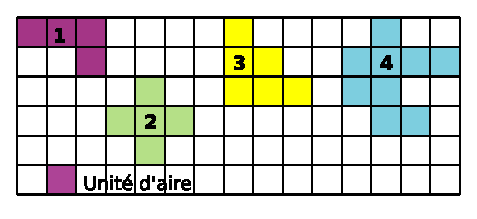
\includegraphics[width=7.2cm]{quadrillageA} \end{center}
\end{exercice}


\begin{exercice}
Détermine l'aire des figures suivantes :

\begin{center} 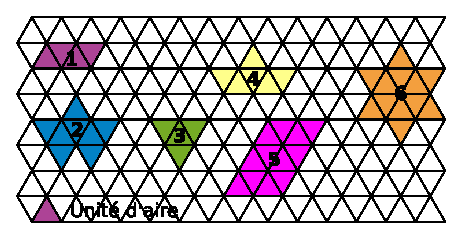
\includegraphics[width=6.9cm]{quadrillageB} \end{center}
\end{exercice}


\begin{exercice}
Détermine l'aire des triangles rectangles suivants :

\begin{center} 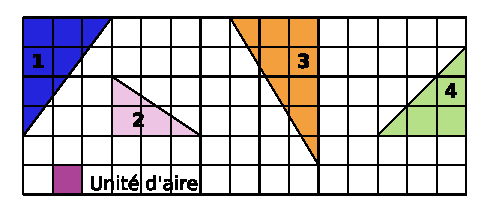
\includegraphics[width=7.2cm]{quadrillageC} \end{center}
\end{exercice}



%%%%%%%%%%%%%%%%%%%%%%%%%%Mise en page
\newpage
%%%%%%%%%%%%%%%%%%%%%%%%%%%%%%%%%%%%%%



\begin{exercice}
Détermine l'aire des triangles suivants :

\begin{center} 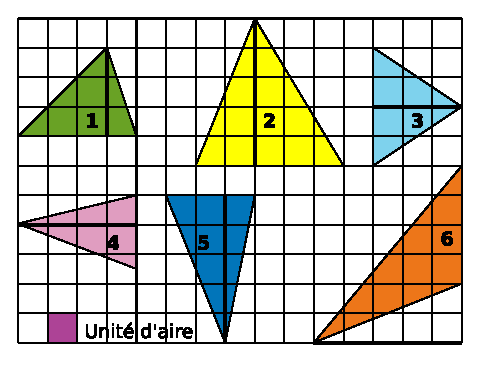
\includegraphics[width=7.2cm]{quadrillageD} \end{center}
\end{exercice}


\begin{exercice}
Détermine l'aire des figures suivantes :

\begin{center} 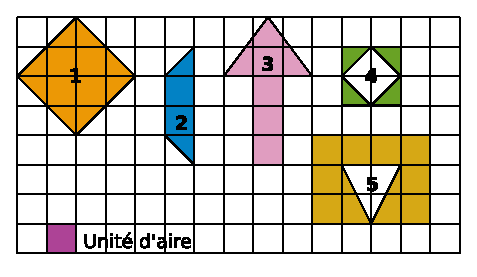
\includegraphics[width=7.1cm]{quadrillageE} \end{center}
\end{exercice}


\begin{exercice}
Détermine le périmètre des figures suivantes :

\begin{center} 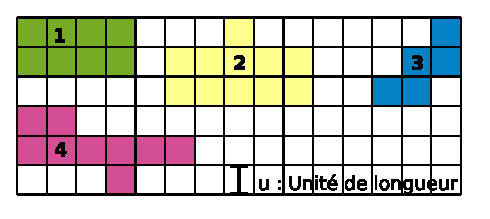
\includegraphics[width=7.1cm]{quadrillageF} \end{center}
\end{exercice}


\begin{exercice}[Avec les carreaux de ton cahier]
\begin{enumerate}
 \item En prenant comme unité d'aire un carreau de ton cahier, réalise trois figures différentes de cinq unités d'aire.
 \item Ces figures ont‑elles le même périmètre ?
 \end{enumerate}
\end{exercice}

\begin{exercice}[Avec les carreaux de ton cahier $(bis)$]
\begin{enumerate}
 \item En prenant comme unité de longueur la longueur d'un carreau de ton cahier, réalise trois figures différentes qui ont un périmètre de douze unités.
 \item Ces figures ont‑elles la même aire ?
 \end{enumerate}
\end{exercice}

\begin{exercice}[Comparaisons]
\begin{enumerate}
 \item Classe ces figures dans l'ordre croissant de leurs aires. Justifie.
 \item Classe ces figures dans l'ordre croissant de leurs périmètres.
 \item La figure qui a la plus grande aire a-t-elle également le plus grand périmètre ?
 \end{enumerate}
\begin{center} 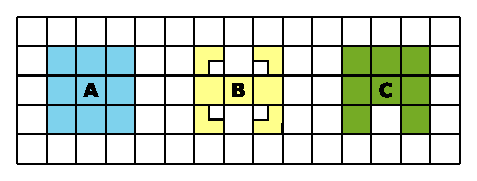
\includegraphics[width=7.1cm]{quadrillageG} \end{center}
\end{exercice}

\begin{exercice}[Aires approximatives]
\begin{center} 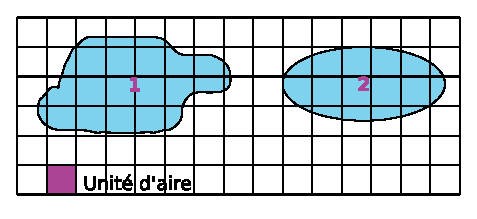
\includegraphics[width=7.2cm]{quadrillageH} \end{center}

Détermine un encadrement de l'aire de chacune des figures.
\end{exercice}


\begin{exercice}[Avec un quadrillage]
Sachant que l'unité d'aire est le carreau, détermine l'aire des figures suivantes en utilisant des aires de triangles :
\begin{center} 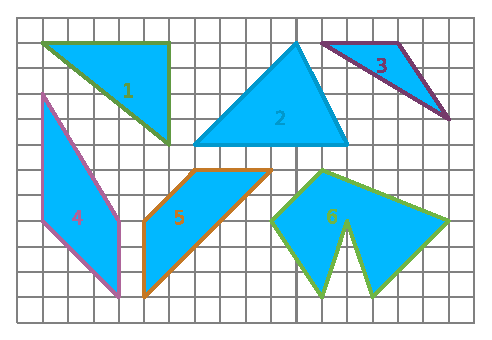
\includegraphics[width=7.1cm]{quadrillageL} \end{center} 
\end{exercice}



%%%%%%%%%%%%%%%%%%%%%%%%%%Mise en page
\newpage
%%%%%%%%%%%%%%%%%%%%%%%%%%%%%%%%%%%%%%



\begin{exercice}[Quadrillage]
\begin{center} 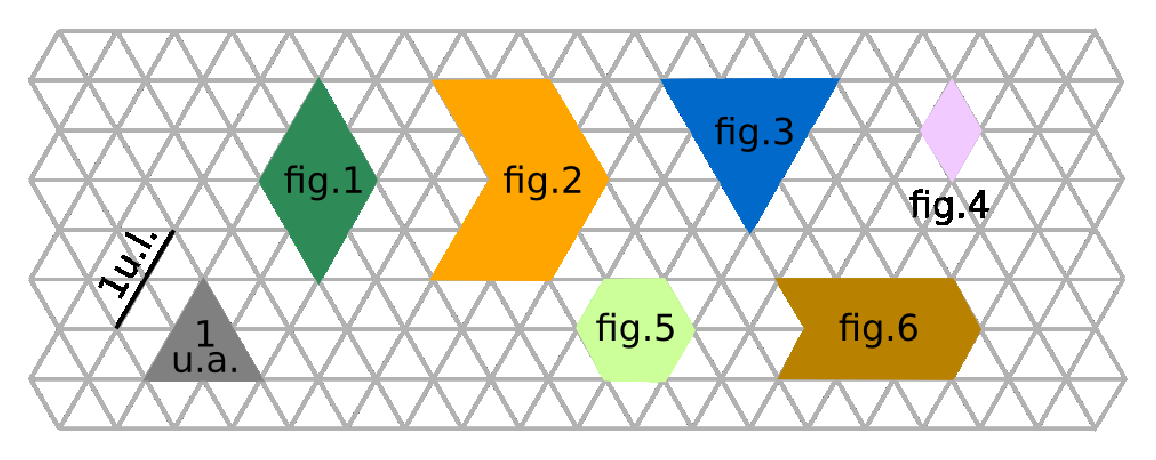
\includegraphics[width=\linewidth]{quadrillageM} \end{center}
\begin{enumerate}
 \item Sur la figure ci-dessus, après avoir observé l’unité de longueur choisie (1 u.l.), détermine le périmètre, en unité de longueur, de chaque figure :
 \begin{CLtableau}{\linewidth}{7}{c}
\hline
\textbf{Figure} & \textbf{1} & \textbf{2} & \textbf{3} & \textbf{4} & \textbf{5} & \textbf{6} \\\hline
\textbf{Périmètre}  & & & & & & \\
exprimé en u.l. & & & & & & \\\hline
 \end{CLtableau} 
 \item Après avoir observé l’unité d’aire choisie (1 u.a.), détermine l’aire, en unités d’aires, de chaque figure :
  \begin{CLtableau}{\linewidth}{7}{c}
\hline
\textbf{Figure} & \textbf{1} & \textbf{2} & \textbf{3} & \textbf{4} & \textbf{5} & \textbf{6} \\\hline
\textbf{Aire} & & & & & & \\
 exprimée en u.a. & & & & & & \\\hline
 \end{CLtableau} 
 \end{enumerate}
\end{exercice}


%%%%%%%%%%%%%%%%%%%%%%%%%%Mise en page
\vspace{1em}
%%%%%%%%%%%%%%%%%%%%%%%%%%%%%%%%%%%%%%




%%%%%%%%%%%%%%%%%%%%%%%%%%%%%%%%%%%%%%%%%%%%%%%%%%%%%%%%%%%%%%%%%%%%

\serie{Avec des formules}


\begin{exercice}[Périmètre et aire du carré]

Recopie et complète le tableau suivant où $c$ est la longueur du côté du carré, $\mathcal{P}$ son périmètre et $\mathcal{A}$ son aire :


\begin{ctableau}{\linewidth}{6}
\hline $c$  & 4 cm & 7 cm & 9 dm & & \\
\hline $\mathcal{P}$ & & & & 32 mm & \\
\hline  $\mathcal{A}$ & & & & & 36 m\up{2} \\
\hline
\end{ctableau}

\end{exercice}


\begin{exercice}[Calcul mental et rectangles]
Les mesures de cinq rectangles sont données en centimètres :

\begin{CLtableau}{\linewidth}{6}{c}
\hline
&  n\up{$\circ$} 1 &  n\up{$\circ$} 2 &  n\up{$\circ$} 3 &  n\up{$\circ$} 4 &  n\up{$\circ$} 5 \\
\hline Longueur & 3 & 5 & 8 & 9 & 8 \\
\hline Largeur & 2 & 3 & 6 & 7 & $1,5$ \\
\hline
\end{CLtableau}


\begin{enumerate}
 \item Calcule le périmètre de chaque rectangle ;
 \item Calcule l'aire de chaque rectangle.
 \end{enumerate}
\end{exercice}


\begin{exercice}[Calcul mental et triangles]
Les mesures des côtés de l'angle droit de cinq triangles rectangles sont données en centimètres :


\begin{cltableau}{\linewidth}{6}
\hline
  &  n\up{$\circ$} 1 & n\up{$\circ$} 2 &  n\up{$\circ$} 3 &  n\up{$\circ$} 4 &  n\up{$\circ$} 5 \\
\hline 1\up{er} côté & 3 & 5 & 8 & 9 & $1,5$ \\
\hline 2\up{ème} côté & 4 & 8 & 5 & 7 & $1,5$ \\
\hline
\end{cltableau}


Calcule l'aire de chaque triangle.
\end{exercice}



\begin{exercice}[Aire de triangles]
Calcule l'aire des différents triangles :
\begin{center} 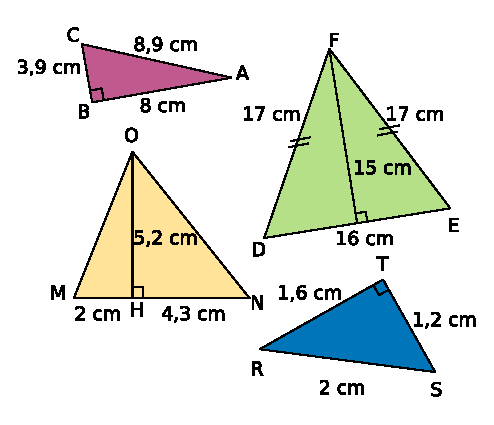
\includegraphics[width=7.6cm]{triangles_differents} \end{center}
\end{exercice}


\begin{exercice}[Aire de triangles rectangles]
Calcule l'aire des triangles rectangles suivants après en avoir fait un croquis :
\begin{enumerate}
 \item $ABC$ rectangle en $A$ tel que $AB = 5$ cm et $AC = 7$ cm ;
 \item $DEF$ rectangle en $E$ tel que $DF = 13$ cm, $DE = 5$ cm et $EF = 12$ cm ;
 \item $MNO$ d'hypoténuse $[MN]$ tel que $MN = 20$ mm, $MO = 12$ mm et $ON = 16$ mm.
 \end{enumerate}
\end{exercice}




%%%%%%%%%%%%%%%%%%%%%%%%%%Mise en page

\vspace*{2cm}

\phantom{Pour sauter une ligne}

\newpage
%%%%%%%%%%%%%%%%%%%%%%%%%%%%%%%%%%%%%%



\begin{exercice}[Périmètre de figures]
En prenant les mesures nécessaires, compare les périmètres des 6 figures ci‑dessous :

\begin{center} 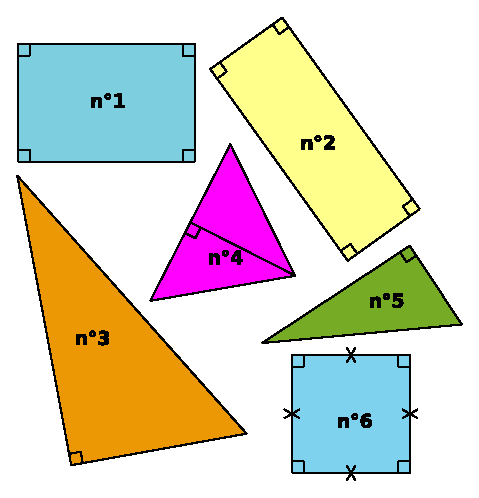
\includegraphics[width=7.4cm]{perimetre_figures} \end{center}
\end{exercice}


\begin{exercice}
Pour chaque parallélogramme, calcule la longueur demandée :
\begin{enumerate}
 \item L'aire du parallélogramme est 36 cm\up{2} et l'un de ses côtés mesure 6 cm. Combien mesure la hauteur relative à ce côté ?
 \item L'aire du parallélogramme est $15,12$ cm\up{2} et l'une de ses hauteurs mesure $3,6$ cm. Combien mesure la base relative à cette hauteur ?
 \end{enumerate}
\end{exercice}


\begin{exercice}[Avec un quadrillage]
Sachant que l'unité d'aire est le carreau, détermine l'aire de chaque figure suivante en utilisant des aires de parallélogrammes :

\begin{center} 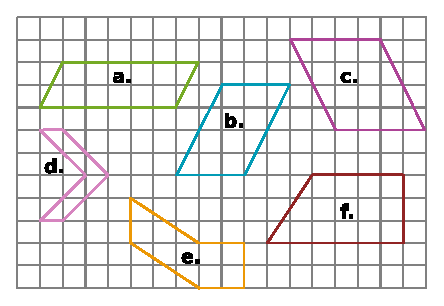
\includegraphics[width=6.6cm]{quadrillageI} \end{center}
\end{exercice}


\begin{exercice}[À main levée…]
\begin{minipage}[c]{0.48\linewidth}
Calcule l'aire et le périmètre de ce parallélogramme tracé à main levée. L'unité de longueur est le centimètre.
 \end{minipage} \hfill%
 \begin{minipage}[c]{0.48\linewidth}
\begin{center} 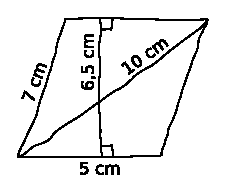
\includegraphics[width=2.9cm]{croquisJ} \end{center} 
  \end{minipage} \\
\end{exercice}


\begin{exercice}
Dans le tableau suivant, $c$ désigne un côté d'un parallélogramme, $h$ la hauteur relative à ce côté et $\mathcal{A}$ l'aire. Quelles sont les valeurs de E, F, G, H et I ? Justifie.

\begin{ltableau}{\linewidth}{3}
\hline
$c$ & $h$ & $\mathcal{A}$ \\\hline
$24$ cm & $8$ cm & E \\\hline
$132$ m & $0,5$ hm & F \\\hline
$16$ mm & G & $64$ mm\up{2} \\\hline
$4,5$ m & H & $14,4$ m\up{2} \\\hline
I & $250$ cm & $7,5$ m\up{2} \\\hline
 \end{ltableau} 
\end{exercice}


\begin{exercice}
Construis un parallélogramme qui a un côté de 6 cm de longueur, un périmètre de 20 cm et une aire de 18 cm\up{2}. Justifie ta construction en indiquant tes calculs.
\end{exercice}


\begin{exercice}[L'un dans l'autre]
\begin{enumerate}
 \item Calcule l'aire de $RATO$, sachant que $RA = 8$ cm et $AT = 6$ cm.
 \begin{center} 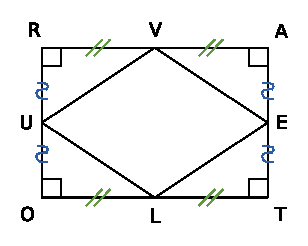
\includegraphics[width=4.2cm]{aireRATO} \end{center} 
 \item Calcule l'aire de $VELU$ de deux façons.
 \end{enumerate}
\end{exercice}


\begin{exercice}
Le quadrilatère $ABCD$ est un rectangle tel que $BC = 4$ cm, $AB = 6$ cm et $K$ est le milieu de $[AD]$. La surface colorée est formée de parallélogrammes accolés. Montre que l'aire de la surface colorée est la moitié de celle du rectangle.
 \begin{center} 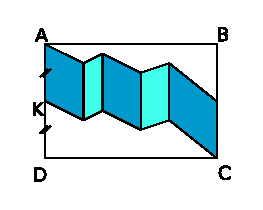
\includegraphics[width=3.6cm]{p_accoles} \end{center} 
\end{exercice}


\begin{exercice}[Pile ou Face ?]
\begin{minipage}[c]{0.38\linewidth}
\includegraphics[width=3cm]{pile_face}
 \end{minipage} \hfill%
 \begin{minipage}[c]{0.58\linewidth}
Le parallélogramme $FACE$ est tel que :
 \begin{itemize}
  \item $EC = 150$ mm ;
  \item $h = 67$ mm ;
  \item $k = 53$ mm.
  \end{itemize}
  \end{minipage} \\
  \begin{enumerate}
   \item Calcule l'aire de $FACE$ ;
   \item Calcule la longueur de la diagonale $[FC]$.
   \end{enumerate}
\end{exercice}


\begin{exercice}[Avec ou sans quadrillage ?]
\begin{minipage}[c]{0.48\linewidth}
\begin{itemize}
 \item Recopie la figure, et partage-la en quatre triangles et un carré. Quelle est alors l'aire du parallélogramme $ABCD$ ?
 \end{itemize}
 \end{minipage} \hfill%
 \begin{minipage}[c]{0.48\linewidth}
\begin{center} \includegraphics[width=3.7cm]{avec_sans} \end{center} 
  \end{minipage} \\
  \begin{itemize}
   \item Pourrais-tu trouver l'aire du parallélogramme $ABCD$ en utilisant seulement le quadrillage de côté $0,5$ cm ? 
   \end{itemize}
\end{exercice}


\begin{exercice}[Deux hauteurs]
\begin{minipage}[c]{0.48\linewidth}
Reproduis sur ton cahier la figure suivante puis trace en rouge la hauteur $[DH]$ et en vert la hauteur relative au côté $[DE]$.
 \end{minipage} \hfill%
 \begin{minipage}[c]{0.48\linewidth}
\begin{center} \includegraphics[width=3.3cm]{croquisFED} \end{center} 
  \end{minipage} \\
\end{exercice}


\begin{exercice}
Calcule l'aire du triangle $ABC$ ci-dessous de trois façons différentes en utilisant les informations données :

\begin{minipage}[c]{0.38\linewidth}
\begin{itemize}
 \item $AB = 12,5$ cm ;
 \item $BC = 20$ cm ;
 \item $AC = 19,5$ cm ;
 \item $CI = 18,72$ cm ;
 \item $AJ = 11,7$ cm ;
 \item $BK = 12$ cm.
 \end{itemize}
 \end{minipage} \hfill%
 \begin{minipage}[c]{0.58\linewidth}
\begin{center} \includegraphics[width=3.6cm]{triangleKIJ} \end{center} 
  \end{minipage} \\
\end{exercice}



%%%%%%%%%%%%%%%%%%%%%%%%%%%%
\vfill
\columnbreak
%%%%%%%%%%%%%%%%%%%%%%%%%%%


\begin{exercice}
Calcule l'aire des triangles suivants. L'unité de longueur est le centimètre :
\begin{colenumerate}{2}
 \item 
 
 \includegraphics[width=3.1cm]{triangleAcm}
  \item 
 
 \includegraphics[width=3.5cm]{triangleBcm}
  \item 
 
 \includegraphics[width=3.3cm]{triangleCcm}
  \item 
 
 \includegraphics[width=3.5cm]{triangleDcm}
 \end{colenumerate}
\end{exercice}


\begin{exercice}
$MNP$ est un triangle de hauteur $[MH]$. Quels sont les valeurs de A, B, C ? Justifie.

\begin{center} \includegraphics[width=2.5cm]{triangleHMNP} \end{center} 

\begin{ltableau}{\linewidth}{3}
\hline
\textbf{$NP$} & \textbf{$MH$} & \textbf{Aire du triangle $MNP$} \\\hline
$7,2$ cm & $4,8$ cm & A \\\hline
B & $3,5$ m & $5,6$ m\up{2} \\\hline
$16$ cm & C & $0,5$ dm\up{2} \\\hline
 \end{ltableau} 
\end{exercice}


\begin{exercice}
Un triangle a pour aire $16,25$ cm\up{2} et l'un de ses côtés mesure $6,5$ cm. Calcule la hauteur relative à ce côté.
\end{exercice}



\begin{exercice}
Un terrain rectangulaire de 45 m de long sur 28 m de large doit être entouré d’une clôture de 3 rangées de fil de fer. On prévoit une ouverture de 4 m de large.
\begin{enumerate}
 \item Quel est le périmètre de ce terrain ?
 \item Quelle est la longueur de fil de fer nécessaire ?
 \item Combien de rouleaux de 100 m de fil de fer faudra-t-il acheter ?
 \item Quelle est l’aire de ce terrain ? Donne la réponse en ares.
 \end{enumerate}
\end{exercice}




\begin{exercice}
Calcule l'aire des deux figures suivantes sans oublier de donner les formules :
\begin{center} \begin{tikzpicture}
%trapèze avec 2 angles droits marqués
\draw (0,0) node[below]{D} -- (7,0) node[below]{C} -- (5.5,3.5) node[above right]{B} -- (0,3.5) node [above left]{A} -- cycle;
\draw (0.2,0)|-(0,0.2);
\draw(0,3.3)-|(0.2,3.5);
\path (0,0) -- (0,3.5) node[midway, left]{3,5 cm};
\path (0,0) -- (7,0) node[midway,below]{7 cm};
\path (0,3.5) -- (5.5,3.5) node[midway,above]{5,5 cm};

\end{tikzpicture}
 \end{center} 
\begin{center} \includegraphics[width=5.8cm]{formule2} \end{center} 
\end{exercice}


\begin{exercice}
Le carré et le rectangle ci-dessous ont le même périmètre.
     
Après avoir fait tous les calculs nécessaires, calcule l’aire du carré.
\begin{center} \includegraphics[width=7.2cm]{carre_rectangle} \end{center} 
\end{exercice}



%%%%%%%%%%%%%%%%%%%%%%%%%%%%%%%%%%%%%%%%%%%%%%%%%%%%%%%%%%%%%%%%%%%%

\end{colonne*exercice}


\exercicesappr
\begin{colonne*exercice}
\begin{exercice}
Calcule le périmètre de la plaque métallique représentée ci‑dessous, puis son aire de deux manières différentes :
\begin{center} \includegraphics[width=3.6cm]{plaque} \end{center}
\end{exercice}

\begin{center}
    \begin{tabular}{|>{\columncolor{J2}}c|}
    \hline
    Rappel : l'aire d'un trapèze est égale à:\\
    $\frac{{(\text{petite base}\, +\, \text{grande base})} \, \times \, {\text{hauteur}}}{2}$.\\
    \hline
\end{tabular}
\end{center}


\begin{exercice}
La figure suivante représente un morceau de tissu. Calcule son aire de deux manières différentes :
\begin{center} \includegraphics[width=4.4cm]{tissu} \end{center}
\end{exercice}


\begin{exercice}
On souhaite entourer, avec du grillage, un jardin carré de 24 m de côté, en laissant une ouverture de 4 m de large. Le grillage choisi coûte 15 CHF le mètre. Quel sera le prix à payer ?
\end{exercice}


\begin{exercice}
M. Albert vend un terrain représenté ci‑dessous au prix de 18 CHF le m\up{2} :
\begin{center} \includegraphics[width=3.7cm]{Albert} \end{center}
Quel est le prix de vente de ce terrain ?
\end{exercice}


\begin{exercice}
Dans une pièce de bois rectangulaire de dimensions $10,2$ cm sur $6,6$ cm, un menuisier découpe un losange dont les sommets se trouvent au milieu de chaque côté du rectangle :
\begin{center} \includegraphics[width=4.6cm]{losange_bois} \end{center}
Calcule l'aire du losange.
\end{exercice}


\begin{exercice}
Sur le mur d’une salle de bains, on a posé 10 rangées de 14 carreaux de 12 cm de côté. Quelle est, en m\up{2}, l’aire de la surface carrelée ?
\end{exercice}


\begin{exercice}
Un rectangle a pour longueur $12,3$ dm et pour largeur $48,5$ cm :
\begin{enumerate}
 \item Calcule le périmètre de ce rectangle en cm puis en dm ;
 \item Calcule l'aire de ce rectangle en cm\up{2} puis en dm\up{2}.
 \end{enumerate}
\end{exercice}


\begin{exercice}[Agrandissement]
Un rectangle a pour dimensions $4,3$ m et $7,8$ m :
\begin{enumerate}
 \item Calcule son périmètre et son aire ;
 \item On double sa largeur et sa longueur.
 
Calcule de nouveau son périmètre et son aire ;
 \item Que constates-tu ?
 \end{enumerate}
\end{exercice}


\begin{exercice}[Même aire]
Construis un carré, un rectangle (non carré) et un triangle rectangle ayant chacun pour aire 16 cm\up{2}.
\end{exercice}


\begin{exercice}[Du rectangle au carré]
\begin{enumerate}
 \item Construis un rectangle de dimensions $5,1$ cm et $3,3$ cm ;
 \item Construis un carré ayant le même périmètre que ce rectangle ;
 \item Le rectangle et le carré ont-ils la même aire ? Explique.
 \end{enumerate}
\end{exercice}


\begin{exercice}
On considère la figure suivante :
\begin{center} \includegraphics[width=6cm]{croquis_grand} \end{center}
\begin{enumerate}
 \item Quelle est la hauteur relative au côté $[CD]$ pour le triangle $ACD$ ?
 \item Calcule l'aire du triangle $ACD$ et la longueur $[BD]$.
 \item Calcule $[AD]$.
 \end{enumerate}
\end{exercice}



%%%%%%%%%%%%%%%%%%%%%%%%%%Mise en page
\newpage
%%%%%%%%%%%%%%%%%%%%%%%%%%%%%%%%%%%%%%




\begin{exercice}[Des rectangles]
Les rectangles $R_1$, $R_2$, $R_3$, $R_4$ et $R_5$ ont tous un périmètre de 20 cm mais des tailles différentes.

\begin{CLtableau}{\linewidth}{6}{c}
\hline 
&  $R_1$ &  $R_2$ & $R_3$ & $R_4$ &  $R_5$ \\ \hline
Longueur d'un côté & \multirow{2}{*}{1} & \multirow{2}{*}{2} & \multirow{2}{*}{3} & \multirow{2}{*}{4} & \multirow{2}{*}{5}  \\
(en cm) &  &  &  &  &  \\ \hline
Longueur de l'autre & & & & & \\
 côté (en cm) & & & & & \\ \hline
 Aire (en cm\up{2}) & & & & & \\ \hline
\end{CLtableau} 

\begin{enumerate}
 \item Reproduis et complète le tableau ci-dessus.
 \item Construis chacun de ces rectangles.
 
Y en a‑t‑il un particulier ? Lequel et pourquoi ?
 \item Dans un tableur, reproduis un tableau similaire à celui‑ci. Fais effectuer les calculs jusqu'au rectangle $R_9$ en allant de $0,5$ cm en $0,5$ cm pour la longueur d'un côté. Tu pourras afficher une représentation graphique de ce tableau. \\[0.5em]
Quel rectangle semble avoir la plus grande aire ?
 \end{enumerate}
\end{exercice}


\begin{exercice}[Quadrilatères inconnus]
Dans chaque cas, construis tous les quadrilatères qui satisfont aux énigmes suivantes :
\begin{enumerate}
 \item Je suis un rectangle. Mes côtés ont des mesures entières. Mon aire est de 18 cm\up{2} et mon périmètre est supérieur à 20 cm. 
 \item Je suis un quadrilatère dont les angles opposés sont égaux deux à deux. Mon aire vaut 24 cm\up{2} et mon périmètre 22 cm. Mes côtés ont des mesures entières.
 \item Je suis un quadrilatère non croisé qui a deux côtés consécutifs égaux et qui possède ses diagonales perpendiculaires. Mon aire vaut 24 cm\up{2}. Mes diagonales ont des mesures entières et se coupent au quart de la plus grande diagonale.
 \end{enumerate}
\end{exercice}



\end{colonne*exercice}

\connaissances


\QCMautoevaluation{Pour chaque question, plusieurs réponses sont proposées. Déterminer celles qui sont correctes.}

\begin{QCM}
  \begin{GroupeQCM}
    \begin{exercice}
    
\begin{center}      \includegraphics[width=1.4cm]{fig1} \includegraphics[width=2.2cm]{fig2}  \end{center}
      \begin{ChoixQCM}{4}
      \item Ces deux figures ont la même aire
      \item Ces deux figures ont le même périmètre
      \item Le périmètre de la figure 2 est plus grand que celui de la figure 1
      \item L'aire de la figure  2 est plus grande que l'aire de la figure 1
      \end{ChoixQCM}
\begin{corrige}
     \reponseQCM{ac} 
   \end{corrige}
    \end{exercice}


    \begin{exercice}
      Mon aire est de 4 cm\up{2} et mon périmètre est de 8 cm. Qui puis‑je être ?
      \begin{ChoixQCM}{4}
      \item Je suis un carré de côté 2 cm
      \item Je suis un rectangle de longueur 3 cm et de largeur 1 cm
      \item Je suis un rectangle de longueur 4 cm et de largeur 1 cm
      \item Je suis un carré de côté 4 cm
      \end{ChoixQCM}
\begin{corrige}
     \reponseQCM{a}
   \end{corrige}
    \end{exercice}
    
    
    \begin{exercice}
      Quelle(s) phrase(s) te semble(nt) raisonnable(s) ?
      \begin{ChoixQCM}{4}
      \item Mesurer la taille d'une fourmi en kilomètres
      \item Mesurer la distance entre deux astres en années‑lumière
      \item Mesurer la longueur d'un fleuve en kilomètres
      \item Mesurer la longueur d'une rue en kilomètres
      \end{ChoixQCM}
\begin{corrige}
     \reponseQCM{bc}
   \end{corrige}
    \end{exercice}


    \begin{exercice}
      814 cm\up{2} est égal à \ldots
      \begin{ChoixQCM}{4}
      \item $81,4$ dm\up{2}
      \item $\numprint{8140}$ mm\up{2}
      \item $\numprint{0,0814}$ m\up{2}
      \item $8,14$ dm\up{2}
      \end{ChoixQCM}
\begin{corrige}
     \reponseQCM{cd}
   \end{corrige}
    \end{exercice}
    
 
    \begin{exercice}
      Une unité adaptée pour exprimer l'aire du terrain d'une maison est \ldots
      \begin{ChoixQCM}{4}
      \item le km\up{2}
      \item l'are
      \item le m\up{2}
      \item le mm\up{2}
      \end{ChoixQCM}
\begin{corrige}
     \reponseQCM{bc}
   \end{corrige}
    \end{exercice}

\end{GroupeQCM}
\end{QCM}
   


\begin{QCM}
  \begin{GroupeQCM}
 
    
    \begin{exercice}
      Pour calculer l'aire d'un triangle rectangle \ldots
      \begin{ChoixQCM}{4}
      \item On multiplie ensemble les deux côtés de l'angle droit
      \item On additionne les longueurs des trois côtés
      \item On divise par 2 le produit des côtés de l'angle droit
      \item On utilise la longueur du plus grand côté
      \end{ChoixQCM}
\begin{corrige}
     \reponseQCM{c}
   \end{corrige}
    \end{exercice}
    
    
    \begin{exercice}
      Quelle(s) est (sont) la (les) phrase(s) vraie(s) ?
      \begin{ChoixQCM}{4}
      \item Si on double le périmètre d'une figure alors on double aussi son aire
      \item L'aire d'un carré de côté $c$ est plus grande que celle d'un disque de diamètre $c$
      \item Si on double l'aire d'une figure alors on double aussi son périmètre
      \item Si on augmente le périmètre d'une figure alors son aire augmente
      \end{ChoixQCM}
\begin{corrige}
     \reponseQCM{b}
   \end{corrige}
    \end{exercice}

\end{GroupeQCM}
\end{QCM}

  


\TravauxPratiques % pour nous "travailler en groupe"

\begin{TP}[La formule de Pick]

On va s'intéresser au théorème de Pick qui permet de calculer l'aire d'un polygone construit sur du papier pointé et dont les sommets sont des points du papier. Voici, par exemple, un tel polygone :
\begin{center} \includegraphics[width=3.8cm]{Pick} \end{center}

\partie{Georg Alexander Pick}
Par groupe, en vous documentant, répondez aux questions suivantes.
\begin{enumerate}
 \item Où et à quelle époque, Georg Alexander Pick a‑t‑il vécu ?
 \item Quels sont les domaines dans lesquels Georg Alexander Pick a travaillé ?
 \item Faites la synthèse des réponses de chaque groupe.
\end{enumerate}

\partie{Formule de Pick}
Pour un polygone construit sur du papier pointé et dont les sommets sont des points du papier, on appelle $N$ le nombre de points situés sur son contour et $P$ le nombre de points situés à l'intérieur. Le théorème de Pick donne la formule pour calculer l'aire $\mathcal{A}$ de ce polygone :
\begin{center} $\mathcal{A} = 0,5 \cdot N + P - 1$ ; l'unité est le carreau. \end{center}
%\vspace{0.5cm}
\begin{enumerate}
 \item Chaque groupe calcule l'aire du rectangle ci‑dessous en utilisant la formule habituelle puis en utilisant la formule de Pick. Comparez avec les réponses des autres groupes. \\[1em]
\begin{center} \includegraphics[width=2.9cm]{Pick2} \end{center}

 \item Chaque groupe construit cinq polygones sur du papier pointé, avec chaque sommet placé sur un point.
 \item Échangez ensuite avec un autre groupe les polygones. Calculez l'aire de chacun des polygones reçus.
 \end{enumerate}
\end{TP}



\pagebreak

\recreation
\begin{enigme}[Invitation au bal]
Sur le carton d'invitation rectangulaire ci-contre, toutes les longueurs sont données en centimètres. Quel est le mot de passe ?
\begin{center} \includegraphics[width=8cm]{invitation} \end{center}
 
 \end{enigme}
 

 



